%%
\widowpenalty1000000
\clubpenalty1000000
% Copyright (c) 2017 - 2019, Pascal Wagler;  
% Copyright (c) 2014 - 2019, John MacFarlane
% 
% All rights reserved.
% 
% Redistribution and use in source and binary forms, with or without 
% modification, are permitted provided that the following conditions 
% are met:
% 
% - Redistributions of source code must retain the above copyright 
% notice, this list of conditions and the following disclaimer.
% 
% - Redistributions in binary form must reproduce the above copyright 
% notice, this list of conditions and the following disclaimer in the 
% documentation and/or other materials provided with the distribution.
% 
% - Neither the name of John MacFarlane nor the names of other 
% contributors may be used to endorse or promote products derived 
% from this software without specific prior written permission.
% 
% THIS SOFTWARE IS PROVIDED BY THE COPYRIGHT HOLDERS AND CONTRIBUTORS 
% "AS IS" AND ANY EXPRESS OR IMPLIED WARRANTIES, INCLUDING, BUT NOT 
% LIMITED TO, THE IMPLIED WARRANTIES OF MERCHANTABILITY AND FITNESS 
% FOR A PARTICULAR PURPOSE ARE DISCLAIMED. IN NO EVENT SHALL THE 
% COPYRIGHT OWNER OR CONTRIBUTORS BE LIABLE FOR ANY DIRECT, INDIRECT, 
% INCIDENTAL, SPECIAL, EXEMPLARY, OR CONSEQUENTIAL DAMAGES (INCLUDING,
% BUT NOT LIMITED TO, PROCUREMENT OF SUBSTITUTE GOODS OR SERVICES; 
% LOSS OF USE, DATA, OR PROFITS; OR BUSINESS INTERRUPTION) HOWEVER 
% CAUSED AND ON ANY THEORY OF LIABILITY, WHETHER IN CONTRACT, STRICT 
% LIABILITY, OR TORT (INCLUDING NEGLIGENCE OR OTHERWISE) ARISING IN 
% ANY WAY OUT OF THE USE OF THIS SOFTWARE, EVEN IF ADVISED OF THE 
% POSSIBILITY OF SUCH DAMAGE.
%%

%%
% This is the Eisvogel pandoc LaTeX template.
%
% For usage information and examples visit the official GitHub page:
% https://github.com/Wandmalfarbe/pandoc-latex-template
%%

\PassOptionsToPackage{unicode=true}{hyperref} % options for packages loaded elsewhere
\PassOptionsToPackage{hyphens}{url}
\PassOptionsToPackage{dvipsnames,svgnames*,x11names*,table}{xcolor}
%
\documentclass[
  a4paper,
  14pt,
  oneside,
  tablecaptionabove
]{scrbook}
\usepackage{lmodern}
\usepackage[shortlabels]{enumitem}
\usepackage{setspace}
\setstretch{1.2}
\usepackage{amssymb,amsmath}
\usepackage{ifxetex,ifluatex}
\ifnum 0\ifxetex 1\fi\ifluatex 1\fi=0 % if pdftex
  \usepackage[T1]{fontenc}
  \usepackage[utf8]{inputenc}
  \usepackage{textcomp} % provides euro and other symbols
\else % if luatex or xelatex
  \usepackage{unicode-math}
  \defaultfontfeatures{Scale=MatchLowercase}
  \defaultfontfeatures[\rmfamily]{Ligatures=TeX,Scale=1}
\fi
% use upquote if available, for straight quotes in verbatim environments
\IfFileExists{upquote.sty}{\usepackage{upquote}}{}
\IfFileExists{microtype.sty}{% use microtype if available
  \usepackage[]{microtype}
  \UseMicrotypeSet[protrusion]{basicmath} % disable protrusion for tt fonts
}{}
%\makeatletter
%\@ifundefined{KOMAClassName}{% if non-KOMA class
%  \IfFileExists{parskip.sty}{%
%    \usepackage{parskip}
%  }{% else
%    \setlength{\parindent}{0pt}
%    \setlength{\parskip}{6pt plus 2pt minus 1pt}}
%}{% if KOMA class
%  \KOMAoptions{parskip=half}}
%\makeatother
\usepackage{xcolor}
\definecolor{default-linkcolor}{HTML}{A50000}
\definecolor{default-filecolor}{HTML}{A50000}
\definecolor{default-citecolor}{HTML}{4077C0}
\definecolor{default-urlcolor}{HTML}{4077C0}
\IfFileExists{xurl.sty}{\usepackage{xurl}}{} % add URL line breaks if available
\IfFileExists{bookmark.sty}{\usepackage{bookmark}}{\usepackage{hyperref}}
\hypersetup{
  pdftitle={Computer-Assisted Language Comparison in Practice},
  pdfborder={0 0 0},
  breaklinks=true}
\urlstyle{same}  % don't use monospace font for urls
\usepackage[margin=2.5cm,includehead=true,includefoot=true,centering]{geometry}
\usepackage[export]{adjustbox}
\usepackage{graphicx}
\usepackage{listings}
\usepackage{makecell}

\newcommand{\passthrough}[1]{#1}

\usepackage{sourcecodepro}
\makeatletter
\defaultfontfeatures[\ttfamily]
       {
        Numbers   = \sourcecodepro@figurestyle ,
        Scale     = \SourceCodePro@scale ,
        Extension = .otf }

    % Monospace font
        \setmonofont
            [ UprightFont    = *-\sourcecodepro@regstyle ,
              ItalicFont     = *-\sourcecodepro@regstyle It ,
              BoldFont       = *-\sourcecodepro@boldstyle ,
              BoldItalicFont = *-\sourcecodepro@boldstyle It ]
            {SourceCodePro}
\makeatother

\usepackage{upquote}
\lstset{ 
    	upquote=true,
    	language=Python,
    	basicstyle=\small\ttfamily,
    	frame=lines,
    	tabsize=4,
    	numbers=left,
    	numberstyle=\tiny,
    	tabsize=2,
    	captionpos=b,
    	%breaklines=true,  
    	%breakatwhitespace=false,
    	escapeinside={\%*}{*)}
}

\usepackage{etoolbox}
\BeforeBeginEnvironment{lstlisting}{\vspace{20pt}\par\noindent\begin{minipage}{\linewidth}}
\AfterEndEnvironment{lstlisting}{\end{minipage}\par\addvspace{\topskip}}
\usepackage{longtable,booktabs}
% Allow footnotes in longtable head/foot
\IfFileExists{footnotehyper.sty}{\usepackage{footnotehyper}}{\usepackage{footnote}}
\makesavenoteenv{longtable}
%\usepackage{graphicx,grffile}
%\makeatletter
%\def\maxwidth{\ifdim\Gin@nat@width>\linewidth\linewidth\else\Gin@nat@width\fi}
%\def\maxheight{\ifdim\Gin@nat@height>\textheight\textheight\else\Gin@nat@height\fi}
%\makeatother
%% Scale images if necessary, so that they will not overflow the page
%% margins by default, and it is still possible to overwrite the defaults
%% using explicit options in \includegraphics[width, height, ...]{}
%\setkeys{Gin}{width=\maxwidth,height=\maxheight,keepaspectratio}
%\setlength{\emergencystretch}{3em}  % prevent overfull lines
%\providecommand{\tightlist}{%
%  \setlength{\itemsep}{0pt}\setlength{\parskip}{0pt}}
%\setcounter{secnumdepth}{-\maxdimen} % remove section numbering
%% Redefines (sub)paragraphs to behave more like sections
%\ifx\paragraph\undefined\else
%  \let\oldparagraph\paragraph
%  \renewcommand{\paragraph}[1]{\oldparagraph{#1}\mbox{}}
%\fi
%\ifx\subparagraph\undefined\else
%  \let\oldsubparagraph\subparagraph
%  \renewcommand{\subparagraph}[1]{\oldsubparagraph{#1}\mbox{}}
%\fi

% Make use of float-package and set default placement for figures to H
\usepackage{float}
\floatplacement{figure}{H}

\ifnum 0\ifxetex 1\fi=0 % if pdftex or luatex
  \usepackage[shorthands=off,main=]{babel}
\else % if xetex
    % See issue https://github.com/reutenauer/polyglossia/issues/127
  \renewcommand*\familydefault{\sfdefault}
    % load polyglossia as late as possible as it *could* call bidi if RTL lang (e.g. Hebrew or Arabic)
  \usepackage{polyglossia}
  \setmainlanguage{english}
\fi

\title{Computer-Assisted Language Comparison in Practice}
\usepackage{etoolbox}
\makeatletter
\providecommand{\subtitle}[1]{% add subtitle to \maketitle
  \apptocmd{\@title}{\par {\large #1 \par}}{}{}
}
\makeatother
\subtitle{Tutorials on Computational Approaches to the History and Diversity of
Languages}
\date{Posts from 2018}
\author{Johann-Mattis List and Tiago Tresoldi (editors)}





%%
%% added
%%

%
% language specification
%
% If no language is specified, use English as the default main document language.
%


%
% for the background color of the title page
%
\usepackage{pagecolor}
\usepackage{afterpage}

%
% TOC depth and 
% section numbering depth
%
\setcounter{tocdepth}{3}

%
% break urls
%
\PassOptionsToPackage{hyphens}{url}

%
% When using babel or polyglossia with biblatex, loading csquotes is recommended 
% to ensure that quoted texts are typeset according to the rules of your main language.
%
\usepackage{csquotes}

%
% captions
%
\definecolor{caption-color}{HTML}{777777}
\usepackage[font={stretch=1.2}, textfont={color=caption-color}, position=top, skip=4mm, labelfont=bf, singlelinecheck=false, justification=raggedright]{caption}
\setcapindent{0em}

%
% blockquote
%
\definecolor{blockquote-border}{RGB}{221,221,221}
\definecolor{blockquote-text}{RGB}{119,119,119}
\usepackage{mdframed}
\newmdenv[rightline=false,bottomline=false,topline=false,linewidth=3pt,linecolor=blockquote-border,skipabove=\parskip]{customblockquote}
\renewenvironment{quote}{\begin{customblockquote}\list{}{\rightmargin=0em\leftmargin=0em}%
\item\relax\color{blockquote-text}\ignorespaces}{\unskip\unskip\endlist\end{customblockquote}}

%
% Source Sans Pro as the de­fault font fam­ily
% Source Code Pro for monospace text
%
% 'default' option sets the default 
% font family to Source Sans Pro, not \sfdefault.
%
\usepackage[default]{sourcesanspro}
\usepackage{sourcecodepro}

% XeLaTeX specific adjustments for straight quotes: https://tex.stackexchange.com/a/354887
% This issue is already fixed (see https://github.com/silkeh/latex-sourcecodepro/pull/5) but the 
% fix is still unreleased.
% TODO: Remove this workaround when the new version of sourcecodepro is released on CTAN.
\ifxetex
\makeatletter
\defaultfontfeatures[\ttfamily]
  { Numbers   = \sourcecodepro@figurestyle,
    Scale     = \SourceCodePro@scale,
    Extension = .otf }
\setmonofont
  [ UprightFont    = *-\sourcecodepro@regstyle,
    ItalicFont     = *-\sourcecodepro@regstyle It,
    BoldFont       = *-\sourcecodepro@boldstyle,
    BoldItalicFont = *-\sourcecodepro@boldstyle It ]
  {SourceCodePro}
\makeatother
\fi

%
% heading color
%
\definecolor{heading-color}{RGB}{40,40,40}
\addtokomafont{section}{\color{heading-color}}
% When using the classes report, scrreprt, book, 
% scrbook or memoir, uncomment the following line.
%\addtokomafont{chapter}{\color{heading-color}}

%
% variables for title and author
%
\usepackage{titling}
\title{Computer-Assisted Language Comparison in Practice}
\author{Johann-Mattis List and Tiago Tresoldi}

%
% tables
%

\definecolor{table-row-color}{HTML}{F5F5F5}
\definecolor{table-rule-color}{HTML}{999999}

%\arrayrulecolor{black!40}
\arrayrulecolor{table-rule-color}     % color of \toprule, \midrule, \bottomrule
\setlength\heavyrulewidth{0.3ex}      % thickness of \toprule, \bottomrule
\renewcommand{\arraystretch}{1.3}     % spacing (padding)

% Reset rownum counter so that each table
% starts with the same row colors.
% https://tex.stackexchange.com/questions/170637/restarting-rowcolors
\let\oldlongtable\longtable
\let\endoldlongtable\endlongtable
\renewenvironment{longtable}{
\rowcolors{3}{}{table-row-color!100}  % row color
\oldlongtable} {
\endoldlongtable
\global\rownum=0\relax}

% Unfortunately the colored cells extend beyond the edge of the 
% table because pandoc uses @-expressions (@{}) like so: 
%
% \begin{longtable}[]{@{}ll@{}}
% \end{longtable}
%
% https://en.wikibooks.org/wiki/LaTeX/Tables#.40-expressions

%
% remove paragraph indention
%
\setlength{\parindent}{0pt}
\setlength{\parskip}{6pt plus 2pt minus 1pt}
\setlength{\emergencystretch}{3em}  % prevent overfull lines

%
%
% Listings
%
%


%
% listing colors
%
\definecolor{listing-background}{HTML}{F7F7F7}
\definecolor{listing-rule}{HTML}{B3B2B3}
\definecolor{listing-numbers}{HTML}{B3B2B3}
\definecolor{listing-text-color}{HTML}{000000}
\definecolor{listing-keyword}{HTML}{435489}
\definecolor{listing-identifier}{HTML}{435489}
\definecolor{listing-string}{HTML}{00999A}
\definecolor{listing-comment}{HTML}{8E8E8E}
\definecolor{listing-javadoc-comment}{HTML}{006CA9}

\lstdefinestyle{eisvogel_listing_style}{
  language         = java,
  numbers          = left,
  xleftmargin      = 2.7em,
  framexleftmargin = 2.5em,
  backgroundcolor  = \color{listing-background},
  basicstyle       = \color{listing-text-color}\small\ttfamily{}\linespread{1.15}, % print whole listing small
  breaklines       = true,
  frame            = single,
  framesep         = 0.19em,
  rulecolor        = \color{listing-rule},
  frameround       = ffff,
  tabsize          = 4,
  numberstyle      = \color{listing-numbers},
  aboveskip        = -0.7em,
  belowskip        = 0.1em,
  abovecaptionskip = 0em,
  belowcaptionskip = 1em,
  keywordstyle     = \color{listing-keyword}\bfseries,
  classoffset      = 0,
  sensitive        = true,
  identifierstyle  = \color{listing-identifier},
  commentstyle     = \color{listing-comment},
  morecomment      = [s][\color{listing-javadoc-comment}]{/**}{*/},
  stringstyle      = \color{listing-string},
  showstringspaces = false,
  escapeinside     = {/*@}{@*/}, % Allow LaTeX inside these special comments
  literate         =
  {á}{{\'a}}1 {é}{{\'e}}1 {í}{{\'i}}1 {ó}{{\'o}}1 {ú}{{\'u}}1
  {Á}{{\'A}}1 {É}{{\'E}}1 {Í}{{\'I}}1 {Ó}{{\'O}}1 {Ú}{{\'U}}1
  {à}{{\`a}}1 {è}{{\'e}}1 {ì}{{\`i}}1 {ò}{{\`o}}1 {ù}{{\`u}}1
  {À}{{\`A}}1 {È}{{\'E}}1 {Ì}{{\`I}}1 {Ò}{{\`O}}1 {Ù}{{\`U}}1
  {ä}{{\"a}}1 {ë}{{\"e}}1 {ï}{{\"i}}1 {ö}{{\"o}}1 {ü}{{\"u}}1
  {Ä}{{\"A}}1 {Ë}{{\"E}}1 {Ï}{{\"I}}1 {Ö}{{\"O}}1 {Ü}{{\"U}}1
  {â}{{\^a}}1 {ê}{{\^e}}1 {î}{{\^i}}1 {ô}{{\^o}}1 {û}{{\^u}}1
  {Â}{{\^A}}1 {Ê}{{\^E}}1 {Î}{{\^I}}1 {Ô}{{\^O}}1 {Û}{{\^U}}1
  {œ}{{\oe}}1 {Œ}{{\OE}}1 {æ}{{\ae}}1 {Æ}{{\AE}}1 {ß}{{\ss}}1
  {ç}{{\c c}}1 {Ç}{{\c C}}1 {ø}{{\o}}1 {å}{{\r a}}1 {Å}{{\r A}}1
  {€}{{\EUR}}1 {£}{{\pounds}}1 {«}{{\guillemotleft}}1
  {»}{{\guillemotright}}1 {ñ}{{\~n}}1 {Ñ}{{\~N}}1 {¿}{{?`}}1
  {…}{{\ldots}}1 {≥}{{>=}}1 {≤}{{<=}}1 {„}{{\glqq}}1 {“}{{\grqq}}1
  {”}{{''}}1
}
\lstset{style=eisvogel_listing_style}

\lstdefinelanguage{XML}{
  morestring      = [b]",
  moredelim       = [s][\bfseries\color{listing-keyword}]{<}{\ },
  moredelim       = [s][\bfseries\color{listing-keyword}]{</}{>},
  moredelim       = [l][\bfseries\color{listing-keyword}]{/>},
  moredelim       = [l][\bfseries\color{listing-keyword}]{>},
  morecomment     = [s]{<?}{?>},
  morecomment     = [s]{<!--}{-->},
  commentstyle    = \color{listing-comment},
  stringstyle     = \color{listing-string},
  identifierstyle = \color{listing-identifier}
}

%
% header and footer
%
\usepackage{fancyhdr}

\fancypagestyle{eisvogel-header-footer}{
  \fancyhead{}
  \fancyfoot{}
  \lhead[]{Computer-Assisted Language Comparison in Practice}
  \chead[]{}
  \rhead[Computer-Assisted Language Comparison in Practice]{}
  \lfoot[\thepage]{}
  \cfoot[]{}
  \rfoot[]{\thepage}
  \renewcommand{\headrulewidth}{0.4pt}
  \renewcommand{\footrulewidth}{0.4pt}
}
\pagestyle{eisvogel-header-footer}

%%
%% end added
%%

\begin{document}

%%
%% begin titlepage
%%

\begin{titlepage}
\newgeometry{left=6cm}
\definecolor{titlepage-color}{HTML}{2D6CA2}
\newpagecolor{titlepage-color}\afterpage{\restorepagecolor}
\newcommand{\colorRule}[3][black]{\textcolor[HTML]{#1}{\rule{#2}{#3}}}
\begin{flushleft}
\noindent
\\[-1em]
\color[HTML]{FFFFFF}
\makebox[0pt][l]{\colorRule[FFFFFF]{1.3\textwidth}{2pt}}
\par
\noindent

{ \setstretch{1.4}
\vfill
\noindent {\huge \textbf{\textsf{Computer-Assisted Language Comparison in Practice}}}
\vskip 1em
{\Large \textsf{Tutorials on Computational Approaches to the History and Diversity of
Languages}}
\vskip 2em
{\large Contributions from 2018}
\vskip 2em
{\large Edited by \\ Johann-Mattis List and Tiago Tresoldi}
\noindent
{\Large \textsf{}
\vfill
{\large Jena, Max-Planck Institute for the Science of Human History}
%\includegraphics[width=\textwidth]{team-logo.pdf}
}

}
\end{flushleft}
\end{titlepage}
\restoregeometry

%%
%% end titlepage
%%



{
\setcounter{tocdepth}{3}
\tableofcontents
\newpage
}
\section*{Introduction}
\phantomsection\addcontentsline{toc}{section}{Introduction (Johann-Mattis List)}
By comparing the languages of the world, we gain invaluable insights
into human prehistory, predating the appearance of written records by
thousands of years. The traditional methods for language comparison are
based on manual data inspection. With more and more data available, they
reach their practical limits. Computer applications, however, are not
capable of replacing experts' experience and intuition. In a situation
where computers cannot replace experts and experts do not have enough
time to analyse the massive amounts of data, a new framework, neither
completely computer-driven, nor ignorant of the help computers provide,
becomes urgent. 
%Such frameworks are well-established in biology and
%translation, where computational tools cannot provide the accuracy
%needed to arrive at convincing results, but do assist humans to digest
%large data sets.

The weblog ``Computer-Assisted Language Comparison in Practice'', published on the Hypotheses platform
for scientific blogging, offers tutorials and discussion notes on computer-assisted approaches to the
history and diversity of languages. A substantial part of its content is contributed as part of the
ERC Starting Grant ``Computer-Assisted Language Comparison'' (CALC, 715618), funded by the European
Research Council. But on the long run, we want to make this blog a platform for everybody willing to
share ideas on small or big problems involving data preparation and analysis in computer-assisted
or computer-based approaches to language comparison.

This document summarizes all contributions from 2018. If you want to cite them, please follow the
instructions at the end of each contribution. I express my gratitude to all contributors, who helped
to make this an interesting collection of tutorials, algorithms, and initial theories
related to the fields of computer-assisted language comparison.

\begin{flushright}
\noindent Johann-Mattis List (Jena, November 2019)
\end{flushright}

\newpage
\section*{Extracting translation data from the Wiktionary project}
\phantomsection\addcontentsline{toc}{section}{Extracting translation data from the Wiktionary
project (Tiago Tresoldi)}

Tiago Tresoldi (11/06/2018)

\emph{Categories}: Dataset

\emph{Tags}: cross-linguistic data formats, lexical data, Wiktionary

\begin{center}\rule{0.5\linewidth}{1pt}\end{center}

\href{https://wiktionary.org}{Wiktionary} is a project for creating a
multilingual, web-based free dictionary of all words in all languages.
Like its sister project \href{https://wikipedia.org}{Wikipedia}, since
its inception it has been subject to criticism both in terms of its
lexicographic approaches and in terms of reliability, content,
procedures, and community operation (see Lepore 2006, Fuertes-Olivera
2009, Meyer 2012). Faults have also been pointed in terms of its
structure which is confusing for newcomers, with parallel and unaligned
information shared among the various language dictionaries, and
differences in accuracy and depth among languages. Notwithstanding, data
from Wiktionary is routinely employed with successful results in natural
language processing and, occasionally, in linguistic research (see Otte
2011, Schlippe 2012, Medero 2009, Li 2012), as it constitutes, by far,
the largest free multilingual lexical source.

The Wikimedia Foundation, the organization managing the project,
releases automatically generated
``\href{https://dumps.wikimedia.org/}{dumps}'' of the data for free and
anonymous download. However, such files cannot be used in linguistic
research without a pre-processing (\enquote{parsing}) stage, as they
constitute more a backup than a data release: in essence, they are XML
files which enclose the textual information of the dictionary articles
(pages potentially holding information for more than one word and more
than one language), which are encoded in the
\href{https://www.mediawiki.org/wiki/Markup_spec}{MediaWiki markup
syntax} (a context-sensitive language that is notoriously difficult to
parse). Data extraction is further complicated by the fact that the
rendered HTML pages include information computed by functions of general
and linguistic scope only available inside an environment running the
Wiktionary server, as well as by Wiktionary collaborators not always
following the project's guidelines and specifications. Many projects
have started to tackle such problems and the difficulties in reusing the
data, including a
\href{https://www.wikidata.org/wiki/Wikidata:Lexicographical_data}{brand
new initiative by Wikidata}.

As such, no standard method for extracting Wiktionary information
exists, with mostly project-specific solutions. An investigation of
parsing tools on GitHub revealed that two main approaches are used:
parsing the XML files and manipulating the entire textual fields, or
parsing the individually rendered HTML pages (fetched either from a
local server or over the Internet). We decided to test a simpler
approach of parsing the dumps as regular text files, reading them line
by line while building an internal structured version of the
information, processing lines with regular expression or simple string
searching methods. The first experiment, whose results are here
presented, involved extracting the parallel translations for English
words found in the English Wiktionary.

The data, based on the dump of 2018-06-01, includes 2,169,063 different
entries from the translation of 149,530 English words and expressions in
2,358 languages (with much variation in vocabulary size among languages:
931 languages have only one entry and German, the largest language after
English, has 97,091 entries). Data is offered in a tabular textual
format, and all entries include (a) a unique ID, (b) a concept ID
referring to the source English word, (c) a description string with the
English source and a short definition (such as ``dictionary/publication
that explains the meanings of an ordered list of words''), (d)
a language ID from the \href{http://glottolog.org}{Glottolog catalog},
(e) the text of the translation as given in the Wiktionary, and (f) an
extra field holding complementary information, when available (such as
phonetic transcription of the text, noun gender, etc.). Data is also
offer in a set of files (tabular textual files, bibtex sources, and JSON
metadata) following the \href{http://cldf.clld.org}{Cross-Linguistic
Data Formats (CLDF)}, a specification designed to allow the exchange of
cross-linguistic data. The code for data extraction is
\href{https://github.com/tresoldi/wiktionary_parser}{available on
GitHub} and the data is available on Zenodo as
\href{https://zenodo.org/record/1286991}``Parallel Translations from the
English Wiktionary'' (DOI: 10.5281/zenodo.1286991). Many thanks to
Johann-Mattis List and to Christoph Rzymski for their help with this
work.

\subsection*{References}

\nopagebreak\hangindent=0.7cm {\small Fuertes-Olivera, Pedro A. (2009). \enquote{The function theory of
lexicography and electronic dictionaries: Wiktionary as a prototype of
collective free multiple-language internet dictionary}. In: H.
Bergenholtz, S. Nielsen, and S. Tarp (eds.), \emph{Lexicography at a
Crossroads: Dictionaries and Encyclopedias Today, Lexicographical Tools
Tomorrow}.  Linguistic Insights: Studies in Language and Communication
90, 99--134. Bern: Peter Lang. }

\nopagebreak\hangindent=0.7cm {\small Lepore, Jill (2006). \enquote{Noah's Mark}. In: \emph{New Yorker},
November 6 2006 Issue. }

\nopagebreak\hangindent=0.7cm {\small Li, Shen; Graça, João V.; Taskar, Ben (2012). \enquote{Wiki-ly
supervised part-of-speech tagging} (PDF). \emph{Proceedings of the 2012
Joint Conference on Empirical Methods in Natural Language Processing and
Computational Natural Language Learning}.  Jeju Island, Korea:
Association for Computational Linguistics. pp.~1389--1398. }

\nopagebreak\hangindent=0.7cm {\small Medero, Julie; Ostendorf, Mari (2009). \enquote{Analysis of vocabulary
difficulty using wiktionary} (PDF). In: \emph{Proc. SLaTE Workshop}.}

\nopagebreak\hangindent=0.7cm {\small Meyer, Christian M.; Gurevych, Iryna (2012). \enquote{Wiktionary: A
new rival for expert-built lexicons? Exploring the possibilities of
collaborative lexicography}. In: Granger, Sylviane; Paquot, Magali,
\emph{Electronic Lexicography}.  Oxford: Oxford University Press. }

\nopagebreak\hangindent=0.7cm {\small Otte, Pim; Tyers, Francis M. (2011). \enquote{Rapid rule-based machine
translation between Dutch and Afrikaans} (PDF). In Forcada, Mikel L.;
Depraetere, Heidi; Vandeghinste, Vincent. \emph{16th Annual Conference
of the European Association of Machine Translation, EAMT11}.  Leuven,
Belgium. pp.~153--160. }

\nopagebreak\hangindent=0.7cm {\small Schlippe, Tim; Ochs, Sebastian; Schultz, Tanja (2012).
\enquote{Grapheme-to-phoneme model generation for Indo-European
languages} (PDF). \emph{Acoustics, Speech and Signal Processing
(ICASSP)}.  Kyoto, Japan. pp.~4801--4804. }

\vskip 2em
\framebox{\tabular{p{0.95\textwidth}}\textbf{Cite this article as}: Tiago Tresoldi, \enquote{Extracting
translation data from the Wiktionary project,} in
\emph{Computer-Assisted Language Comparison in Practice},  11/06/2018,
\url{https://calc.hypotheses.org/32}.\endtabular}

\newpage
\section*{Exporting sublists from a wordlist with LingPy and Concepticon}
\phantomsection\addcontentsline{toc}{section}{Extracting sublists from a wordlist with LingPy and Concepticon (Johann-Mattis List)}

Johann-Mattis List (16/07/2018)

\emph{Categories}: Code

\emph{Tags}: code example, concept list, Concepticon, LingPy, sublist,
Swadesh list

\begin{center}\rule{0.5\linewidth}{1pt}\end{center}

When dealing with linguistic datasets, we may often want to export only
a small part of our data, for example, only vocabulary in a certain
range, such as the
\href{http://concepticon.clld.org/contributions/Swadesh-1952-200}{Swadesh
list of 200 items} or the
\href{http://concepticon.clld.org/contributions/Yakhontov-1991-35}{list
of 35 items by Yakhontov} (originally published in
\href{http://bibliography.lingpy.org?key=Starostin1991}{Starostin 1991})
. Thanks to the \passthrough{\lstinline!pyconcepticon!} API and LingPy's
built-in export functions for wordlists, this task can be done just in a
few lines of code, as we will see below. If you prefer to see the raw
code instead of the step-by-step explanation below, you can find a
GitHub Gist
\href{https://gist.github.com/LinguList/7804cb127e74a9263b4eab9c5af4bc6f}{here}.


In order to get started, I work with a dataset that was originally
published along with a paper by
\href{http://bibliography.lingpy.org?key=Kolipakam2018}{Kolipakam et al.
(2018)}. This dataset can be downloaded from the supplemental material
accompanying the paper, and the important file is a zip-folder called
\href{http://rsos.royalsocietypublishing.org/highwire/filestream/18890/field_highwire_adjunct_files/3/rsos171504supp4.zip}{SI\_robustness\_cognate\_coding.zip},
from which you have to extract the file
\passthrough{\lstinline!DravLex.tsv!}. I take this dataset, since it is
published, it is easy to get a copy of the data, and the data has been
already linked to Concepticon, although not officially in Version 1.1,
but you can already receive the data from our
\href{https://github.com/clld/concepticon-data}{GitHub} repository,
where the concept list is labelled
\href{https://github.com/clld/concepticon-data/blob/master/concepticondata/conceptlists/Kolipakam-2018-100.tsv}{Kolipakam-2018-100},
following our Concepticon naming convention, which takes the first
author, the year of the publication, and the number of items in order to
create a stable identifier for a concept list.

To get started, you need to make sure that you have the
\lstinline!pyconcepticon! API installed in its most recent version. You
should find all important instructions for this on the GitHub repository
of the Concepticon project (see
\href{https://github.com/clld/concepticon-data}{clld/concepticon-data}). You also need to have LingPy installed in its current 2.6 version
(ideally also make sure to take the most recent version from our GitHub
repository: \href{https://github.com/lingpy/lingpy}{lingpy/lingpy}).
Equipped with this information and the dataset, open a terminal in the
folder in which you have placed the file \lstinline!DravLex.tsv! , and
start by loading LingPy and the \lstinline!pyconcepticon! API.

\begin{lstlisting}
[IN ]: from pyconcepticon.api import Concepticon
[IN ]: from lingpy import *
\end{lstlisting}

This is of course easy, but now we will process the concept list of
Kolipakam et al. and try to extract those items which we can also find
in the very short list of 35 items by Yakhontov. In order to do so, you
need to understand how Concepticon stores data in the Python API, and
this may be somewhat confusing at the first sight, since the class
hierarchy is created in such a way that it directly reflects the online
version of the Concepticon and makes extensive use of dictionaries (more
precisely \lstinline!OrderedDict!). But let's start step by step, and
first, we simply load the API:

\begin{lstlisting}
[IN ]: CNC = Concepticon()
\end{lstlisting}

And now we load the concept lists by Yakhontov and Kolipakam:

\begin{lstlisting}
[IN ]: yakhontov = CNC.conceptlists['Yakhontov-1991-35']
[IN ]: kolipakam = CNC.conceptlists['Kolipakam-2018-100']
\end{lstlisting}

What is important here is the structure of the \lstinline!Conceptlist!
objects that we just loaded. They all have an attribute
\lstinline!concepts! , which is itself a dictionary with the identifier
of a given concept as key, and a \lstinline!Concept! object as value.
The \lstinline!Concept! object itself has again different attributes,
and the most important attributes for us are the
\lstinline!concepticon_id! and the \lstinline!english! entry. We need
the \lstinline!english! attribute of the data by Kolipakam et al. to
determine the Concepticon identifiers in the dataset, since the dataset
itself does not officially link the data to Concepticon. We use the
Concepticon identifiers to compare which of the concept sets in the
Dravidian data also occur in Yakhontov's list. We start by slightly
modifying our two lists (\lstinline!yakhontov! and
\lstinline!kolipakam!) first, and then extract a sublist with English
glosses from them:

\begin{lstlisting}
[IN ]: yakhontov = [c.concepticon_id for c in yakhontov.concepts.values()]
[IN ]: kolipakam = [(c.concepticon_id, c.english) for c in  kolipakam.concepts.values()]
[IN ]: sublist = [english for english, concepticon_id in kolipakam if concepticon_id in yakhontov]
[IN ]: print('Overlap shows {0} items in common.'.format(len(sublist))) 
[OUT]: Overlap shows 31 items in common.
\end{lstlisting}

We can now load the \lstinline!DravLex.tsv! file and output it in such a
way that only a subset of concepts is selected which occur in our
sublist. For this, we use the \lstinline!output!-method of the
\lstinline!Wordlist! class in LingPy, but in contrast to the normal
output procedure, we specify a subset and a condition. Since the
condition is evaluated internally in form of Python code passed to
LingPy, this looks a bit ugly, as we define a dictionary that specifies
columns that occur in the wordlist, and these columns' content is then
checked against the Python code that we pass as string, but it is the
fastest way to accomplish this task in LingPy:

\begin{lstlisting}
[IN ]: wl = Wordlist('DravLex.tsv')
[IN ]: wl.output('tsv', filename='DravLex-sublist', subset=True, rows={"concept": "in "+str(sublist)})
\end{lstlisting}

That's all we have to do. In order to verify that we really exported
only a part of the wordlist, we can reload it and count its basic
parameters (number of languages, concepts, and words):

\begin{lstlisting}
[IN ]: wl2 = Wordlist('DravLex-sublist.tsv') 
[IN ]: print('{0}:{1} languages, {2}:{3} concepts, and {4}:{5} words'.format(wl.width, wl2.width, wl.height, wl2.height, len(wl), len(wl2))) 
[OUT]: 20:20 languages, 100:31 concepts, and 2114:660 words
\end{lstlisting}

Another way to achieve this goal which has the advantage of allowing you
to circumvent to write the data to file and reload it is to create a new
wordlist object from the original wordlist object. In order to do so, we
create a dictionary with integers as key where the key 0 reflects the
header of the wordlist object and the keys link to values that are a
list, just as we know it from the normal wordlist objects.

\begin{lstlisting}
[IN ]: D = {0: [c for c in wl.columns]}
\end{lstlisting}

We can fill this now still empty dictionary by iterating over all
entries in our original wordlist and checking whether the concepts occur
in our sublist:

\begin{lstlisting}
[IN ]: for idx, concept in wl.iter_rows('concept'):
......     if concept in sublist:
......         D[idx] = [entry for entry in wl[idx]] 
\end{lstlisting}

This dictionary can then directly be passed to the \lstinline!Wordlist!
class and loaded in the same way in which we would load a normal
wordlist.

\begin{lstlisting}
[IN ]: wl2 = Wordlist(D)
\end{lstlisting}

We can again quickly verify that this yields the same expected output.

\begin{lstlisting}
[IN ]: print('{0}:{1} languages, {2}:{3} concepts, and {4}:{5} words'.format(wl.width, wl2.width, wl.height, wl2.height, len(wl), len(wl2))) 
[OUT]: 20:20 languages, 100:31 concepts, and 2114:660 words
\end{lstlisting}

Which of the methods to use depends on personal preferences and also the
task at hand. It may be preferable to load a sublist on the fly and
manipulate it further in LingPy, and it may be useful to save it to
file, which is faster with our subset option in LingPy's output function
for wordlists. When playing a bit with the conditions, many more things
can be done in order to manipulate wordlist objects within Python,
without having to manipulate them manually, or by writing wordlist
content to other datatypes in order to handle them with additional
libraries, like, for example, Pandas. The only problem is, at least in
my experience, that it seems to be difficult for users to grasp the
major concepts behind this practice in LingPy, as they have been
developed long before tools like Pandas were common ways of manipulating
arrays and tabular data.

\subsection*{References}

\nopagebreak\hangindent=0.7cm {\small Kolipakam, V., F. Jordan, M. Dunn, S. J. Greenhill, R. Bouckaert, R.
Gray, and A. Verkerk (2018): ``A Bayesian phylogenetic study of the
Dravidian language family.'' \emph{Royal Society Open Science} 5.171504.
1-17. }

\nopagebreak\hangindent=0.7cm {\small Starostin, S. (1991): ``Altajskaja problema i
proischoždenije japonskogo jazyka {[}The Altaic problem
and the origin of the Japanese language{]}.'' Nauka: Moscow.}

\vskip 2em
\framebox{\tabular{p{0.95\textwidth}}\textbf{Cite this article as}: Johann-Mattis List, \enquote{Exporting
Sublists from a Wordlist with LingPy and Concepticon,} in
\emph{Computer-Assisted Language Comparison in Practice},  16/07/2018,
\url{https://calc.hypotheses.org/58}.\endtabular}

\newpage

\section*{Cooking with CLICS}
\phantomsection\addcontentsline{toc}{section}{Cooking with CLICS (Johann-Mattis List)}

Johann-Mattis List (08/08/2018)

\emph{Categories}: Code, Dataset

\emph{Tags}: CLICS, colexification network, Concepticon, example

\begin{center}\rule{0.5\linewidth}{1pt}\end{center}

\href{https://github.com/xrotwang/}{Robert Forkel} just published a very
nice
\href{https://github.com/clics/clics2/tree/master/cookbook}{cookbook
example} for our CLICS database (\href{http://bibliography.lingpy.org?key=List2018f}{List et al. 2018f},
\url{http://clics.clld.org}), where you can find out how to manipulate
the data further, apart from just installing it and running it to
replicate our analyses.

This cookbook tells you how the underlying SQLITE database is structured
and how you can, after \href{https://github.com/clics/clics2}{installing
CLICS} and the respective packages, access the data to conduct studies
of your own.

As a little example of what you can do with the new CLICS API, let me
illustrate in this post, how we can use the old CLICS data (underlying
the version 1.0 by
\href{http://bibliography.lingpy.org?key=List2014f}{List et al. 2014},
\url{http://clics.lingpy.org}), available from
\href{https://github.com/clics/clics1}{here}, in the new application,
specifically the standalone that we provide.


In order to get started, we begin by installing the
\href{https://github.com/clics/clics2}{pyclics} API. For this, I assume
that Python3 is installed in a recent version on our system, along with
\lstinline!pip! the command for downloading and installing new packages,
and the version-control system \lstinline!git! .

In order to install the \lstinline!pyclics! API, simply type the
following in your terminal:

\begin{lstlisting}
$ git clone https://github.com/clics/clics2
$ cd clics2
$ pip install -e .
\end{lstlisting}

Now, you can install the old CLICS data underlying version 1.0.

\begin{lstlisting}
$ pip install -e git+https://github.com/clics/clics1.git@v1.1#egg=lexibank_clics1
\end{lstlisting}

In addition, you need to install \lstinline!pyglottolog! and
\lstinline!pyconcepticon! , but not with \lstinline!pip! , but rather as
local clones (as you need to know where they are installed. So we
recommend to install both packages by opening your terminal in your
preferred folder (ideally the one where you installed
\lstinline!pyclics!).

\begin{lstlisting}
$ cd ..
$ git clone https://github.com/clld/concepticon-data
$ cd concepticon-data
$ pip install -e .
$ cd ..
$ git clone https://github.com/clld/glottolog
$ pip install -e .
$ cd ..
\end{lstlisting}

Now you can load the data into your personal CLICS database by simply
typing:

\begin{lstlisting}
$ clics load ./concepticon-data ./glottolog
\end{lstlisting}

In order to calculate the colexification network, just type:

\begin{lstlisting}
$ clics -t 2 colexification
\end{lstlisting}

In order to create a standalone application for the data which you can
put on a server or browse (when using Firefox as webbrowser) even
locally, type:

\begin{lstlisting}
$ clics -t 2 communities
$ clics -t 3 subgraph
\end{lstlisting}

You will find the application in the path \lstinline!clics2/app/! . Just
click on the file \lstinline!index.html! and open it, and you can see an
interface that reminds of the old \enquote{look-and-feel} of CLICS.

\begin{figure}[htb]
\centering
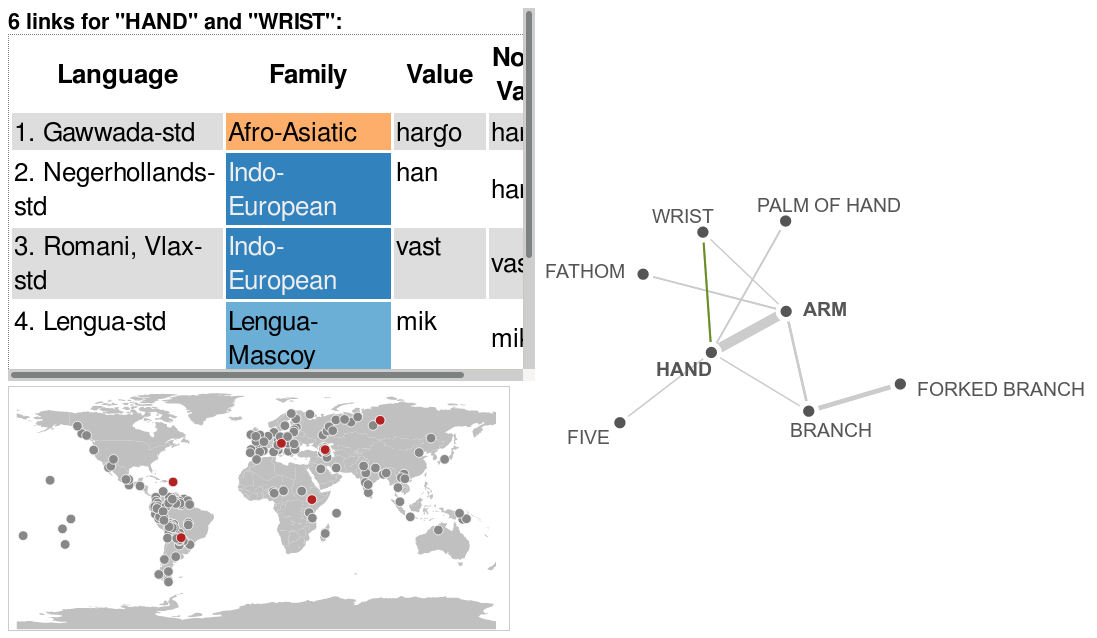
\includegraphics[width=\textwidth]{images/clics-local.png}
\captionsetup{justification=centering}
\caption*{\small \textbf{Figure 1}: Local CLICS application.}
\end{figure}

If you want to have a closer look at the network without following all
the code examples above, you can also directly access it at
\url{http://calc.digling.org/clics1}, where we have uploaded the
version that we created ourselves in order to test this example.

\subsection*{References}

\nopagebreak\hangindent=0.7cm {\small List, J.-M., T. Mayer, A. Terhalle, and M. Urban (eds.) (2014):
{CLICS: Database of Cross-Linguistic Colexifications}.  Version
1.0. Forschungszentrum Deutscher Sprachatlas: Marburg.
\url{http://www.webcitation.org/6ccEMrZYM}.
}

\nopagebreak\hangindent=0.7cm {\small List, J.-M., S. J. Greenhill, C. Anderson, T. Mayer, T. Tresoldi, and R.
Forkel (eds.) (2018): {CLICS: Database of Cross-Linguistic
Colexifications}.  Max Planck Institute for the Science of Human
History: Jena. }

\vskip 2em
\framebox{\tabular{p{0.95\textwidth}}\textbf{Cite this article as}: Johann-Mattis List, \enquote{Cooking with
CLICS,} in \emph{Computer-Assisted Language Comparison in Practice}, 
08/08/2018, \url{https://calc.hypotheses.org/384}.\endtabular}
\newpage

\section*{Representing structural data in CLDF}
\phantomsection\addcontentsline{toc}{section}{Representing structural data in CLDF (Johann-Mattis List)}


Johann-Mattis List (03/09/2018)

\emph{Categories}: Code, Dataset

\emph{Tags}: CLDF, cross-linguistic data formats, Python, structural
dataset

\begin{center}\rule{0.5\linewidth}{1pt}\end{center}

The Cross-Linguistic Data Formats initiative (CLDF,
\url{https://cldf.clld.org},
\href{http://bibliography.lingpy.org?key=Forkel2018}{Forkel et al. 2018}) has helped a lot in preparing the CLICS² database of cross-linguistic
colexifications (\url{https://clics.lingpy.org},
\href{http://bibliography.lingpy.org?key=List2018e}{List et al. 2018}),
since linking our data to Concepticon (\url{https://concepticon.clld.or},
\href{http://bibliography.lingpy.org?key=List2016xxx}{List et al. 2016}) and Glottolog (\url{https://glottolog.org},
\href{http://bibliography.lingpy.org?key=Hammarstroem2018}{Hammarström
et al. 2018}) has provided incredible help in merging the different
datasets into a big comparative dataset.

CLDF, however, is not restricted to lexical data, but can also be
successfully used to store structural data, although --- due to the
nature of structural data --- it is much more difficult to compare
different datasets.
 
In a recent publication by
\href{http://bibliography.lingpy.org?key=Szeto2018}{Szeto et al. 2018}
the authors use structural data to compare different Chinese dialect
varieties typologically. The data itself is provided in the paper, but
unfortunately, the authors do not share it in form of text files, but
list it in tables in the original publication. They also do not share
the NEXUS file they created in order to analyze the data with the
Neighbor-net algorithm (\href{http://bibliography.lingpy.org?key=Bryant2004}{Bryant and Moulton
2004}) implemented by the SplitsTree software package (\href{http://bibliography.lingpy.org?key=Huson1998}{Huson 1998}).

Thanks to the help of David Morrison, who extracted the presence-absence
matrix from the table in the original paper, I was now able to convert
their data to the CLDF format for structural datasets. The data is
available via GitHub at
\href{https://github.com/cldf-datasets/szetosinitic}{cldf-datasets/szetosinitic}.
The folder contains both the \enquote{raw} data that I used (a KML-file
with the dialect locations submitted as supplement to the paper, as well
as the feature matrix extracted by David Morrison, and the parameter
description as typed off by myself), as well as the CLDF data, and a
script that converts the raw data into CLDF. In addition, I have added a
script that converts the data to a NEXUS file that can be directly read
into SplitsTree. Robert Forkel furthermore added automatic tests that
will be carried out if users propose changes to the GitHub repository by
making a pull request.

In order to test the code for these different conversions, you can
simply clone (=download) the data with git:

\begin{lstlisting}
$ git clone https://github.com/cldf-datasets/szetosinitic
\end{lstlisting}

Afterwards, you should install the dependencies, as listed in the file
\lstinline!pip-requirements.txt! (make sure you use Python3 for this
task, as Python2 is not supported):

\begin{lstlisting}
$ pip install -r pip-requirements.txt
\end{lstlisting}

Once this is done, you can test the conversion of the raw data into the
CLDF data by typing:

\begin{lstlisting}
$ python chinese.py
\end{lstlisting}

This won't give you any visual feedback, but it will in fact recreate
all the CLDF data in the folder \lstinline!cldf! , and it was the way I
created the CLDF data in a first instance.

To receive the NEXUS file, just type:

\begin{lstlisting}
$ python nexus.py
\end{lstlisting}

This will read the CLDF data that you just created and write it in NEXUS
format ot the file \lstinline!chinese.nex! .

To illustrate that one can use this basic procedure for more than just
one dataset, I added an older and smaller dataset published by
\href{http://bibliography.lingpy.org?key=Normal2003}{Norman (2003)}
which I happened to have typed off quite some time before. This dataset
can be found on GitHub at
\href{https://github.com/cldf-datasets/normansinitic}{cldf-datasets/normansinitic}
and you can follow exactly the same steps in order to convert this data
as well into NEXUS format.

In the future, I hope we can provide more functionality in the CLDF
package itself, so that people could use the \lstinline!cldf! command
that is installed as well if you install the \lstinline!pycldf! package,
to convert a dataset from CLDF to different formats needed for
computations. However, given the diversity of formats, with very
different flavors of NEXUS being required by different software
packages, we should better wait a bit until we have extracted the most
important use cases that can be encountered.

\subsection*{References}

\nopagebreak\hangindent=0.7cm {\small Bryant, D. and V. Moulton (2004): {Neighbor-Net} {. An
agglomerative method for the construction of phylogenetic networks}. 
\emph{Molecular Biology and Evolution} 21.2. 255-265. }

\nopagebreak\hangindent=0.7cm {\small Forkel, R., J.-M. List, S. J. Greenhill, C. Rzymski, S. Bank, M. Cysouw,
H. Hammarström, M. Haspelmath, G. Kaiping, and R. Gray (forthcoming):
{Cross-Linguistic Data Formats, advancing data sharing and re-use
in comparative linguistics}.  \emph{Scientific Data}. }

\nopagebreak\hangindent=0.7cm {\small Hammarström, H., R. Forkel, and M. Haspelmath (2018):
{Glottolog}.  Version 3.3. Max Planck Institute for Evolutionary
Anthropology: Leipzig. }

\nopagebreak\hangindent=0.7cm {\small Huson, D. (1998): {SplitsTree: analyzing and visualizing
evolutionary data}.  \emph{Bioinformatics} 14.1. 68-73. }

\nopagebreak\hangindent=0.7cm {\small List, J.-M., M. Cysouw, and R. Forkel (2016): {Concepticon. A
resource for the linking of concept lists}.  In: {Proceedings of
the Tenth International Conference on Language Resources and Evaluation}
. 2393-2400. }

\nopagebreak\hangindent=0.7cm {\small List, J.-M., S. J. Greenhill, C. Anderson, T. Mayer, T. Tresoldi, and R.
Forkel (2018): {CLICS². An improved database of cross-linguistic
colexifications assembling lexical data with help of cross-linguistic
data formats}.  \emph{Linguistic Typology} 22.2. 277-306. }

\nopagebreak\hangindent=0.7cm {\small Norman, J. (2003): {The Chinese dialects} {. Phonology}
. In: Thurgood, G. and R. LaPolla (eds.): {The Sino-Tibetan
languages}.  Routledge: London and New York. 72-83. }

\nopagebreak\hangindent=0.7cm {\small Szeto, P., U. Ansaldo, and S. Matthews (2018): {Typological
variation across Mandarin dialects: An areal perspective with a
quantitative approach}.  \emph{Linguistic Typology} 22.2. 233-275. }

\vskip 2em
\framebox{\tabular{p{0.95\textwidth}}\textbf{Cite this article as}: Johann-Mattis List, \enquote{Representing
Structural Data in CLDF,} in \emph{Computer-Assisted Language Comparison
in Practice},  03/09/2018, \url{https://calc.hypotheses.org/445}.\endtabular}

\newpage
\section*{A fast implementation of the Consonant Class Matching method
for automatic cognate detection in LingPy}
\phantomsection\addcontentsline{toc}{section}{A fast implementation of the Consonant Class Matching method
for automatic cognate detection in LingPy (Johann-Mattis List)}



Johann-Mattis List (01/10/2018)

\emph{Categories}: Code

\emph{Tags}: cognate detection, consonant class matching method,
implementation, LexStat, LingPy, sound classes

\begin{center}\rule{0.5\linewidth}{1pt}\end{center}

LingPy's \lstinline!LexStat! class for cognate detection confuses those
who want to apply it, since the name of the Python class is the same as
the name of one of the methods the class provides, but the class can be
used for other types of cognate detection as well. I recommend all users
of LingPy that they give a read to our most recent tutorial on LingPy's
cognate detection method (\href{http://bibliography.lingpy.org?key=List2018d}{List et al. 2018}),
since the three most important methods are discussed there in detail,
namely the edit distance method for cognate detection, which makes use
of the simple, normalized edit distance, the SCA method, based on the
Sound-Class-Based Alignment algorithm (\href{http://bibliography.lingpy.org?key=List2014d}{List 2014}), and
the LexStat method (ibid.). Applying these methods in LingPy is fairly
simple and described in detail in our aforementioned tutorial. But
LingPy offers an additional method for cognate detection that has the
advantage of being extremely fast and thus especially suitable for
exploratory data analysis of very large datasets. This method is called
\lstinline!turchin! in LingPy, named after the first author of a paper
presenting the method (\href{http://bibliography.lingpy.org?key=Turchin2010}{Turchin et al.
2010}), but the method itself, which Turchin et al. name
\enquote{Consonant Class Matching} method, goes originally back to
\href{http://bibliography.lingpy.org?key=Dolgopolsky1964}{Dolgopolsky
(1964)}), and has long since been implemented as a part of the STARLING
software package (\href{http://starling.rinet.ru/program.php?lan=en}{http://starling.rinet.ru/program.php}).

The method is fairly simple. For a given wordlist with a certain number
of concepts translated into a certain number of languages, all words are
converted to consonant classes, following either Dolgopolsky's original
proposal (Dolgopolsky 1964) or later modifications (\href{http://bibliography.lingpy.org?key=Kassian2015b}{Kassian et al.
2015}). After conversion, only the first two consonants of each word
are compared, and the basic rule is that if two words match in their
first two consonant classes, they should be considered as cognate.
Attentive readers may now immediately ask: What do you do if words don't
have a consonant? To handle cases like this, the method has two specific
additional rules to convert a word to its first two consonant classes.
The first rule says that words starting with a vowel will be treated as
if they started with a glottal stop and thus assigned the consonant
class \enquote{H}. The second rule, which is not often mentioned in the
literature, is that, if a word consists of only one vowel, the second
consonant will also be rendered as a \enquote{H}.

Whether this is a good idea or not, is in fact not important. Previous
tests have shown that the method in general does not yield too many
false positives, but instead may miss many good cognates (\href{http://bibliography.lingpy.org?key=List2017c}{List et al. 2017}).
That means that the method is rather \emph{conservative}, at least as
long as it is applied to words within the same concept slot. Even more
important than its conservative behaviour (as linguists we always prefer
false negatives over false positives), however, is that the method is
extremely fast, and its complexity is linear: the amount of time we need
to cluster words into cognate sets with the Consonant Class Matching
method is directly proportional to the number of words in our sample.
The reason for this is that the cognate-match criterion of the CCM
method is transitive: if word A has the same consonant classes as word
B, and word C has the same consonant classes as word B, word C must also
have the same consonant classes as word A.

We can also say: the criterion by which we partition a couple of words
into cognate sets is just their consonant classes themselves. The
consonant classes can be directly used as the labels for the resulting
clusters, since the criterion of cognate set assignment is identity in
those classes. As a result, we can compute the clusters by simply
computing the consonant classes per word in our data, which explains why
the complexity is linear.

The problem with the \lstinline!turchin! method in the
\lstinline!LexStat! class of LingPy is that the implementation is
\emph{not} linear in terms of complexity, since it internally uses a
distance matrix for all word pairs in a slot in which words that are
cognate according to the CCM criterion are given the distance 0 and the
other words are given the distance 1. This distance matrix is then
analysed with the UPGMA algorithm (\href{http://bibliography.lingpy.org?key=Sokal1958}{Sokal and Michener
1958}) or one of the other luster approaches offered by LingPy. While
this will still be fast, since the clusters are always well-balanced,
the method may easily break if you try to identify cognates across, say,
1000 languages with 200 concepts for each of them. This is not only due
to the matrix-implementation in LingPy (which is not needed and was
created in a time when I did not see that the CCM method has a linear
solution), but also due to the complex operations and conversions that
are done whenever you load a dataset into LingPy's \lstinline!LexStat!
class.

Writing a workaround is in fact very easy, and presenting this
workaround is exactly what I want to do in this blogpost. My hope is
that we manage to add this to the next official release of LingPy so
that users can profit from the very fast computation of cognate sets for
large dataset, without having to wait for hours until the normal LexStat
approaches yield (at times disappointing) results. In the following, I
will illustrate in a step-by-step guide how cognate sets can be inferred
with a linear implementation of the CCM method.

To get started, we import the LingPy library.

\begin{lstlisting}
from lingpy import *
\end{lstlisting}

We then load our wordlist, which can be any wordlist in LingPy or CLDF
format (\href{http://bibliography.lingpy.org?key=Forkel2018a}{Forkel et
al. 2018}). I will be lazy in this test and simply import the data from
\href{http://bibliography.lingpy.org?key=Kessler2001}{Kessler (2001)},
which is available from LingPy's test suite.

\begin{lstlisting}
from lingpy.tests.util import test_data
wl = Wordlist(test_data('KSL.qlc'))
\end{lstlisting}

We then make a function that converts a given tokenized sound sequence
to its first two consonant classes, following the criteria mentioned
above.

\begin{lstlisting}
def to_ccm(tokens):
    cv = tokens2class(tokens, 'cv')
    cl = tokens2class(tokens, 'dolgo')
    dolgo = ''
    if cv[0] == 'V': 
        dolgo += 'H'
    else:
        dolgo += cl[0]
    for c, v in zip(cv[1:], cl[1:]):
        if c == 'C':
            dolgo += v
    if len(dolgo) == 1:
        dolgo += 'H'
    return dolgo[:2]
\end{lstlisting}

Now we just add a new column to our wordlist, but instead of adding only
consonant classes, we add the concepts as well, since we want to make
sure that cognates are only assigned inside a given concept slot. For
this, we use the \lstinline!Wordlist.add_entries! method, which can
combine the information given in two and more columns and add it to a
new column (but this application is a bit tricky and needs some practice
if one wants to use it correctly).

\begin{lstlisting}
wl.add_entries(
    'cog', 
    'tokens,concept', 
    lambda x, y : x[y[1]]+'-'+to_ccm(x[y[0]]))
\end{lstlisting}

Having calculated a new column that contains the name of the concept for
each word plus its sound classes, we can conveniently use the
\lstinline!Wordlist.renumber! function in LingPy to convert the data in
this column to integers. Note that we use the \lstinline!override!
keyword, since the original data already contains cognate sets in a
column called \lstinline!cogid! .

\begin{lstlisting}
wl.renumber('cog', override=True)
\end{lstlisting}

To see whether we succeded, let us at the same time compute a little
tree from the data. Don't be scared: since Kessler's data contains
unrelated languages, and we use a very crude algorithm for cognate
detection, the result will show a tree for the languages, even if there
is no evidence for their relatedness.

\begin{lstlisting}
wl.calculate('tree', ref='cogid')
\end{lstlisting}

Last not least, we print the tree in Ascii-Art on the terminal:

\begin{lstlisting}
print(wl.tree.asciiArt())
\end{lstlisting}

And the result will look like this:

\begin{lstlisting}
                    /-Navajo
          /edge.0--|
         |          \-Turkish
-root----|
         |          /-Hawaiian
         |         |
          \edge.4--|                    /-English
                   |          /edge.1--|
                   |         |          \-German
                    \edge.3--|
                             |          /-Albanian
                              \edge.2--|
                                        \-French
\end{lstlisting}

Obviously, this method should not be used to avoid that experts code or
check the cognates, but it may turn out to be very useful for studies
that want to quickly explore the signal in a certain dataset, and check
whether it is worthwhile to compare a given set of languages further. In
the future, I hope that I will find time to add this implementation of
the CCM method to the lingpy package, to make it even easier for
interested scholars to use it on their data.

\subsection*{References}

\nopagebreak\hangindent=0.7cm {\small Dolgopolsky, A. (1964): {Gipoteza drevnejšego rodstva
jazykovych semej Severnoj Evrazii s verojatnostej točky zrenija} {[}A
probabilistic hypothesis concering the oldest relationships among the
language families of Northern Eurasia{]}. \emph{Voprosy Jazykoznanija}
2. 53-63.}

\nopagebreak\hangindent=0.7cm {\small Forkel, R., J.-M. List, S. J. Greenhill, C. Rzymski, S. Bank, M. Cysouw,
H. Hammarström, M. Haspelmath, G. Kaiping, and R. Gray (forthcoming):
{Cross-Linguistic Data Formats, advancing data sharing and re-use
in comparative linguistics}.  \emph{Scientific Data}. . }

\nopagebreak\hangindent=0.7cm {\small Kassian, A., M. Zhivlov, and G. Starostin (2015):
{Proto-Indo-European-Uralic comparison from the probabilistic
point of view}.  \emph{The Journal of Indo-European Studies} 43.3-4.
301-347. }

\nopagebreak\hangindent=0.7cm {\small Kessler, B. (2001): {The significance of word lists} {.
Statistical tests for investigating historical connections between
languages}.  CSLI Publications: Stanford. }

\nopagebreak\hangindent=0.7cm {\small List, J.-M. (2014): {Sequence comparison in historical
linguistics}.  Düsseldorf University Press: Düsseldorf. }

\nopagebreak\hangindent=0.7cm {\small List, J.-M., S. J. Greenhill, and R. Gray (2017): {The potential
of automatic word comparison for historical linguistics}.  \emph{PLOS
ONE} 12.1. 1-18. }

\nopagebreak\hangindent=0.7cm {\small List, J.-M. , M. Walworth, S. J. Greenhill, T. Tresoldi, and R.
Forkel (2018): {Sequence comparison in computational historical
linguistics}.  \emph{Journal of Language Evolution}. 3 (2). 130-144.\\ }

\nopagebreak\hangindent=0.7cm {\small Sokal, R. and C. Michener (1958): {A statistical method for
evaluating systematic relationships}.  \emph{University of Kansas
Scientific Bulletin} 28. 1409-1438. 2.3. 130-144.\\ }

\nopagebreak\hangindent=0.7cm {\small Turchin, P., I. Peiros, and M. Gell-Mann (2010): {Analyzing
genetic connections between languages by matching consonant classes}. 
\emph{Journal of Language Relationship} 3. 117-126. }

\vskip 2em
\framebox{\tabular{p{0.95\textwidth}}\textbf{Cite this article as}: Johann-Mattis List, \enquote{A fast
implementation of the Consonant Class Matching method for automatic
cognate detection in LingPy,} in \emph{Computer-Assisted Language
Comparison in Practice}, 01/10/2018,
\url{https://calc.hypotheses.org/477}.\endtabular}

\newpage
\section*{Enhancing morphological annotation for internal language
comparison}
\phantomsection\addcontentsline{toc}{section}{Enhancing morphological annotation for internal langauge
comparison (Nathanael E. Schweikhard)}

Nathanael E. Schweikhard (10/10/2018)

\emph{Categories}: Annotation

\emph{Tags}: EDICTOR, morphological annotation, standardization

\begin{center}\rule{0.5\linewidth}{1pt}\end{center}

In language { comparison, } there is a long history of using
concept-based wordlists to get insights into the degree of similarity
between languages, going back at least to Morris Swadesh (Swadesh 1950).
For these purposes, words from different languages that share the same
meaning are compared, either manually or with computational methods. The
latter have the advantages of being both faster and more consistent.
However, there are also limits to what computer-based methods can detect
for the time being.

One of the biggest problems in this context is that none of the
currently available methods for automatic cognate detection can infer
partial cognates directly if no information on morpheme boundaries is
provided by the user. As a result, if morpheme boundaries are missing
and morphological differences are frequent in the data one wants to
investigate, automatic cognate detection can be seriously hampered
(List, Greenhill, and Gray 2017).

\begin{figure}[htb]
\centering
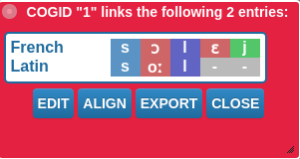
\includegraphics[width=0.45\textwidth]{images/graphic-1.png}
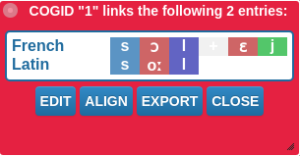
\includegraphics[width=0.45\textwidth]{images/graphic-2.png}
\captionsetup{justification=centering}
\caption*{\small \textbf{Figure 1}: Screenshots from EDICTOR (List 2017) contrasting
automatic sound alignment without and with morphological annotation.}
\end{figure}

For example, Latin \emph{sōl} /soːl/ and French \emph{soleil} /sɔlɛj/
(both \enquote{sun}) would be considered more similar by an algorithm if
it \enquote{knew} that the French word can be analyzed as consisting of
two morphemes, and that it should only consider the first one, i. e.
/sɔl/. It might also be the case that the same morphemes appear as
allomorphs within a given language, e. g. due to vowel harmony or
umlaut, but currently there are no automatic methods to detect
allomorphic variation inside a language.

In order to tackle these problems one could either try to use existing
methods for automatic morpheme boundary detection (Creutz and Lagus
2005) to preprocess our linguistic datasets, or one could increase the
information that is made available to the algorithms in order to enable
them to compare morphemes instead of full words (Hill and List 2017;
List, Lopez, and Bapteste 2016).

Given that automatic morpheme detection does not yield reliable results
at the moment, especially not for small wordlists as they are typically
used in historical linguistics, we are currently trying to formalize the
second approach by developing standards and examples for best practice
to augment wordlists with morphological information. In doing so, we do
not only hope to optimize our annotation frameworks in order to
establish a workflow for future annotations, but also to create example
annotations for future tests of novel methods for automatic morpheme
detection.

Our goal here is to explore the possibilities of integrating any kind of
morphological structures, be they synchronic or diachronic, within a
consistent annotation framework. In the following, I want to give a
short overview on some new ideas we came up with during the last months.

\subsection*{Preliminaries of annotation}

We established a standardized way of how the data needs to be prepared
and formatted, following the standard input formats of LingPy (List,
Greenhill, and Forkel 2017) and EDICTOR (List 2017), which are largely
compatible with the format specifications laid out by the CLDF
initiative (Forkel et al. 2018). This is necessary to guarantee the
comparability of the results, the re-usability of helper scripts, the
integrability with existing annotation solutions, and
machine-readability in general. The format specification requires that
the wordlists are turned into a spreadsheet saved as TSV-file with a
header row and one row for each wordform. The column containing this
data is titled FORM. For each other kind of information, a distinct
column is used. It needs to be made sure that each field contains only a
single string of characters (including spaces if phrases occur among the
data), and not multiple forms. If the data with which one is working
does not follow these requirements or if other corrections to it are
needed, they need to be adjusted accordingly. The original data is
always preserved in the column VALUE, so nothing is lost (unless one
excludes a given word form completely from the comparison). Comments and
notes explaining some specific aspects of the entries under question are
placed in the column NOTE.

The first column is called ID and contains a consecutive integer ID that
needs to be larger than zero.~This is necessary in order to further
refine the data with the help of EDICTOR (List 2017) and has the
additional advantage of making it easy to put the rows back into the
original order if they were reordered. Since several languages might be
included in one file and we want to allow for language-external
comparison as well, the language of the data is specified in the column
DOCULECT (following the terminology of Good and Cysouw 2013). Wordlists
are typically created with the use of elicitation glosses and those are
included in a column given the header CONCEPT.

\begin{table}[h]
\resizebox{\textwidth}{!}{ % use resizebox with \textwidth
\centering
\begin{tabular}[c]{@{}llllll@{}}
\toprule
\textbf{{ ID }}
 &
\textbf{{ DOCULECT}}
 &
\textbf{{ CONCEPT}}
 &
\textbf{{ VALUE}}
 &
\textbf{{ FORM }}
 &
\textbf{{ NOTE }}
\tabularnewline
{ 147 }
 &
{ Old High German }
 &
{ the goat }
 &
{ geiz }
 &
{ geiz }
 &
\tabularnewline
{ 148 }
 &
{ Old High German }
 &
{ the he-goat }
 &
{ boc, buc }
 &
{ boc }
 &
\tabularnewline
{ 149 }
 &
{ Old High German }
 &
{ the kid }
 &
{ zickîn }
 &
{ zickîn }
 &
\tabularnewline
{ 150 }
 &
{ Old High German }
 &
{ the horse }
 &
{ (h)ros }
 &
{ hros }
 &
\tabularnewline
{ 151 }
 &
{ Old High German }
 &
{ the stallion }
 &
{ hengist }
 &
{ hengist }
 &
{ wrong meaning }
\tabularnewline
{ 152 }
 &
{ Old High German }
 &
{ the stallion }
 &
 &
{ reino }
 &
{ correction}
\tabularnewline
{ 153 }
 &
{ Old High German }
 &
{ the mare }
 &
{ meriha }
 &
{ meriha }
 &
\tabularnewline
{ 154 }
 &
{ Old High German }
 &
{ the foal or colt }
 &
{ folo }
 &
{ folo }
 &
\tabularnewline
{ 155 }
 &
{ Old High German }
 &
{ the donkey }
 &
{ esil }
 &
{ esil }
 &
\tabularnewline
{ 156 }
 &
{ Old High German }
 &
{ the mule }
 &
{ mûl }
 &
{ mûl }
 &
\tabularnewline
\bottomrule
\end{tabular}
} % resize box
\captionsetup{justification=centering}
\caption*{\small \textbf{Table 1:} Entries from the Old High German wordlist of the World
Loanword Database (Haspelmath 2009) prepared for further annotation.}
\end{table}


Especially when using one's own data it is highly recommended to also
add a column with the Concepticon-ID (List et al. 2018, see also
\url{https://concepticon.clld.org}) corresponding to the elicitation
gloss in order to make sure that later comparison across different
datasets will be facilitated.

\subsection*{Segmented IPA-transcriptions}

After these preliminary preparations, the words are turned into
sequences of IPA-characters. This facilitates comparing languages since
the original spelling is often quite idiosyncratic and several
computational analyses which one might want to use the data for are only
possible if it is provided in IPA. In order to create IPA from
orthographic sources, there are different possibilities: One could
convert all orthographic entries to their IPA version manually, one
could try to extract the data from an available database that lists
phonetic transcriptions for orthographic entries (as many modern
dictionaries do), or one could write an orthography profile (see Moran
and Cysouw 2018, and for an introduction to how to create this kind of
file see
\href{http://htmlpreview.github.io/?https://raw.githubusercontent.com/digling/calc-seminar/master/handouts/Session_6.html}{this
tutorial}) and convert the data with help of the Python implementation
provided by the \href{https://github.com/cldf/segments}{segments
package}. 

Unfortunately, orthography profiles only work for very regular
orthographies like those used by field workers who for convenience
transcribe languages in alphabetic letters. For orthographies with a
longer history, orthography profiles often cannot be used, since the
orthography does not contain full information on the pronunciation. For
example, in German, vowel length is not always marked by the spelling.
Therefore for these kinds of spelling systems, one of the other options
or a combination thereof needs to be chosen.

The IPA-column is named TOKENS. This is the default name for it in
EDICTOR. Also, the individual sounds (all sounds that are judged as a
sound unit by the researcher, i.e., including affricates and diphthongs,
depending on the language under investigation) are separated by spaces.

\subsection*{Standardizing annotation
practice}

After all these previous (and at times tedious) steps of data
preparation, we can finally start to annotate the morphemes in our data
by marking morpheme borders with a plus sign. Here again this can either
be done manually or by using some computer-assisted approach. If common
morphemes are known to the researcher, a very simple (but in our
experience also efficient) approach for marking at least a larger part
of the morphemes semi-automatically is to use search and replace
functionalities (in combination with regular expressions if needed). In
this way, nearly all instances of, for example, the German prefix \{
\emph{ver} \} can be easily annotated by searching for { \^{}f ɛ r } and
replacing it with { f ɛ r + } (the { \^{} } marks that it must be at the
beginning of a word). Afterwards it is necessary to go through the whole
list manually to check for erroneously segmented instances and add those
morphemes that have not been caught with the automatic procedure. The
resulting annotated data is left in the column TOKENS, but for the
un-annotated IPA a backup-column could be created and it is useful to
add a column for notes.

\begin{table}
\resizebox{\textwidth}{!}{%
\begin{tabular}[c]{@{}lllll@{}}
\toprule
\textbf{{ ID }} & \textbf{{ DOCULECT }} & \textbf{{ CONCEPT }} &
\textbf{{ FORM }} & \textbf{{ TOKENS }}\tabularnewline
{ 632 } & { German } & { rotten } & { verfault } & { f ɛ r + f a ʊ l + t
}\tabularnewline
{ 633 } & { German } & { rotten } & { vermodert } & { f ɛ r + m oː d ə r
+ t }\tabularnewline
{ 634 } & { German } & { drink } & { trinken } & { t r ɪ ŋ k + ə n
}\tabularnewline
{ 635 } & { German } & { hunger } & { Hunger } & { h ʊ ŋ ə r
}\tabularnewline
{ 636 } & { German } & { famine } & { Hungersnot } & { h ʊ ŋ ə r + s + n
oː t }\tabularnewline
{ 637 } & { German } & { thirst } & { Durst } & { d ʊ r s t
}\tabularnewline
{ 638 } & { German } & { suck } & { saugen } & { z au g + ə n
}\tabularnewline
{ 639 } & { German } & { chew } & { kauen } & { k au + ə n
}\tabularnewline
{ 640 } & { German } & { swallow } & { schlucken } & { ʃ l ʊ k + ə n
}\tabularnewline
{ 641 } & { German } & { swallow } & { verschlucken } & { f ɛ r + ʃ l ʊ
k + ə n }\tabularnewline
\bottomrule
\end{tabular}}
\captionsetup{justification=centering}
\caption*{\small \textbf{Table 2:} Entries from the German wordlist of the
Intercontinental Dictionary Series (Key and Comrie 2015), in IPA with
morpheme borders.}
\end{table}

Once the data has been annotated in this way, we follow an idea proposed
in Hill and List (2017) by adding glosses to the morphemes. This helps
us specifically to disambiguate homophone morphemes which do not go back
to the same ancestor, and, of course, this step can also be done at the
same time when correcting the initial morpheme boundaries. The glosses
are added into a column called MORPHEMES. The form is free: which words
to use as a gloss for a morpheme depends only on practicality, as long
as the entry does not have any spaces (as EDICTOR segments the MORPHEMES
content by spaces). What is important, however, is that identical
morphemes across different words are given the same gloss, and that
those that are not identical are given different glosses. In our tests,
we use English as our glossing language and derive the morpheme gloss
from the main meaning of each given word. Thus, German \{ \emph{nah} \}
(\enquote{near}), for example, is glossed as NEAR. In cases when there
are more homonyms in the language investigated than in English, we
recommend to add \_B, \_C etc. to the glosses to distinguish them
consistently. In contrast to the very free form proposed in Hill and
List (2017), we have made good experience in writing content morphemes
in upper case in order to mark them visually. Glosses for grammatical
morphemes on the other hand are written in lower case and start with an
underscore. Thus, we write { \_infinitive } for the infinitive suffix in
our German test data. This is based on a new feature of the EDICTOR, by
which all morpheme glosses preceded by an underscore are displayed in
transparent and small font to further mark the different in status for
grammatical and content morphemes. Additionally, the underscore can be
quickly added or deleted by right-clicking on a morpheme in the
interface.

Distinguishing content from grammatical forms is not always an easy
task, and at it is likely that scholars will disagree about individual
decisions. To base our annotations on a clear-cut criterion, we
considered as content morphemes only those that appear also as free
morphemes or that are confixes (e. g. \emph{Schwieger} -,
\enquote{-in-law}). But the definition of a free morpheme as well as the
border between a confix and an affix is far from clear and free
morphemes can also be grammatical. Similarly, it is also not always
clear where to put a morpheme border as definitions of what is a
morpheme vary and may depend on the research question or the information
available. Ideally, one would use the same criterion for glossing not
only throughout the same, but also across different languages, but this
may prove to be difficult in practice since problems with the definition
might only be noticed during the course of annotation. In order to
reduce the amount of typing, a script can again be used to find and
annotate the most common morphemes. All data, however, will usually need
to be checked manually, since it is not possible to distinguish
automatically between homophonous and recurring morphemes.

\subsection*{Deeper levels of
annotation}

As mentioned above, not only morpheme borders but also allomorphs should
be included in the information provided to the computer. These
non-homophone cognates can be marked in the MORPHEMES column during the
previous step by giving them the same gloss names but differentiating
them with a number at their end. So \{ \emph{näh} \} in German
\emph{näherkommen} (\enquote{approach}) is glossed in our examples in
Table 3 below as NEAR2. In a further step, we annotate the actual roots
by adding a column that we call ROOTS and one that we call ROOTIDS,
where we no longer distinguish between NEAR and NEAR2. Although this
annotation may seem rather complex, it has the clear advantage that it
allows us to distinguish different kinds of word families inside the
same language, namely those where morphemes recur in the same, and those
where they recur in different forms (be it due to allophony or internal
sound change).

\begin{table}
\resizebox{\textwidth}{!}{%
\begin{tabular}[c]{@{}lllllllll@{}}
\toprule
\textbf{{ ID }} & \textbf{{ CONCEPT }} &
\textbf{{ FORM }} & \textbf{{ TOKENS }} & \textbf{{ MORPHEMES }} &
\textbf{{ COGIDS }} & \textbf{{ ROOTS }} & \textbf{{ ROOTIDS
}}\tabularnewline
{ 1239 } & { approach } & { nahen } & { n aː + ə n } & {
NEAR \_infinitive } & { 953 42 } & { NEAR \_infinitive } & { 890 42
}\tabularnewline
{ 1240 } & { approach } & { hingehen } & { h ɪ n + g eː + ə
n } & { TO GO \_infinitive } & { 926 441 42 } & { TO GO \_infinitive } &
{ 865 414 42 }\tabularnewline
{ 1241 } & { approach } & { näherkommen } & { n ɛː + ə r +
k ɔ m + ə n } & { NEAR2 \_comp COME \_infinitive } & { 954 130 955 42 }
& { NEAR \_comp COME \_infinitive } & { 890 128 891 42 }\tabularnewline
{ 1242 } & { approach } & { sich nähern } & { z ɪ x \_ n ɛː
+ ə r + n } & { ONESELF NEAR2 \_comp \_infinitive2 } & { 414 954 130 329
} & { \_reflexive NEAR \_comp \_infinitive } & { 394 890 128 42
}\tabularnewline
{ 1243 } & { enter } & { hineingehen } & { h iː n + ai n +
g eː + ə n } & { TO IN GO \_infinitive } & { 926 389 441 42 } & { TO IN
GO \_infinitive } & { 865 371 414 42 }\tabularnewline
{ 1244 } & { enter } & { eintreten } & { ai n + t r eː t +
ə n } & { IN TREAD \_infinitive } & { 389 933 42 } & { IN TREAD
\_infinitive } & { 371 872 42 }\tabularnewline
{ 1245 } & { enter } & { hereinkommen } & { h ɛ r + ai n +
k ɔ m + ə n } & { FROM IN COME \_infinitive } & { 939 389 940 42 } & {
FROM IN COME \_infinitive } & { 878 371 152 42 }\tabularnewline
{ 1246 } & { carry (bear) } & { tragen } & { t r aː g + ə n
} & { CARRY \_infinitive } & { 956 42 } & { CARRY \_infinitive } & { 436
42 }\tabularnewline
{ 1247 } & { carry (bear) } & { schleppen } & { ʃ l ɛ p + ə
n } & { CARRY\_B \_infinitive } & { 957 42 } & { CARRY\_B \_infinitive }
& { 892 42 }\tabularnewline
\bottomrule
\end{tabular}}
\captionsetup{justification=centering}
\caption*{\small \textbf{Table 3:} Entries from the German wordlist of the
Intercontinental Dictionary Series (Key and Comrie 2015) with
morphological glosses and root annotation.}
\end{table}

\subsection*{What we cannot do yet}

Morphological annotation works with strings of characters and predefined
fields. This means that some types of information which one might want
to include are difficult to implement. For an etymological annotation in
which not only transparent morpheme borders are included, one will
likely encounter cases in which morpheme borders have become fuzzy due
to phonological mergers. An example would be the German word
\emph{Messer} (/mɛsɐ/, \enquote{knife}) which in modern German is
monomorphemic but goes back to a compound (Old High German
\emph{mezzi-sahs}, later \emph{mezzi-rahs}, literally
\enquote{food-knife}, see Watkins 1990: 295). For some languages, cases
like these can be found even when taking a synchronic perspective.

Additionally, it would be interesting to include information on the
kinds of sound changes that a morpheme or word underwent during its
history. But we have not decided where to add this information, and how
to standardize it, specifically also because it will be difficult to
find a principled and standardized way to do so across different
languages. If there was only one sound shift per morpheme, it would be
quite possible to develop a straightforward proposal for annotation, but
considering that morphemes are not limited in the amount of phonological
changes they may accumulate, we find it difficult to come up with a
proposal at this stage of the research. However, since we annotate
allomorphs consistently, we are already able to identify all allomorphs
of a given root in our data. Therefore, it will be easy to add
information on sound changes later, once we managed to find a useful
representation format.

Finally, we could not (yet) find any systematic way to model analogical
relations between words. Given the importance and frequency of analogy
in arguments in historical linguistics, we will try to come up with
proposals for this in future versions of our annotation framework.

\subsection*{References}

\nopagebreak\hangindent=0.7cm {\small Creutz, M., and K. Lagus. 2005. \enquote{Unsupervised Morpheme
Segmentation and Morphology Induction from Text Corpora Using Morfessor
1.0.} Publications in Computer and Information Sciences 81. Helsinki:
Helsinki University of Technology. }


\nopagebreak\hangindent=0.7cm {\small Forkel, Robert, Johann-Mattis List, Simon J. Greenhill, Christoph
Rzymski, Sebastian Bank, Michael Cysouw, Harald Hammarström, Martin
Haspelmath, Gereon A. Kaiping, and Russell D. Gray. 2018.
\enquote{Cross-Linguistic Data Formats, Advancing Data Sharing and
Re-Use in Comparative Linguistics.} \emph{Nature Scientific Data}. }


\nopagebreak\hangindent=0.7cm {\small Good, Jeff, and Michael Cysouw. 2013. \enquote{Languoid, Doculect,
Glossonym: Formalizing the Notion of \enquote{Language}.} \emph{Journal
of Language Documentation and Conservation} 7: 331--59.
\url{https://scholarspace.manoa.hawaii.edu/handle/10125/4606}. }

\nopagebreak\hangindent=0.7cm {\small Haspelmath, Martin, and Uri Tadmor, eds. 2009. \emph{WOLD}.  Leipzig:
Max Planck Institute for Evolutionary Anthropology.
\url{https://wold.clld.org/}. }

\nopagebreak\hangindent=0.7cm {\small Hill, Nathan W., and Johann-Mattis List. 2017. \enquote{Challenges of
Annotation and Analysis in Computer-Assisted Language Comparison: A Case
Study on Burmish Languages.} \emph{Yearbook of the Poznań Linguistic
Meeting}, no. 3: 47--76. }

\nopagebreak\hangindent=0.7cm {\small Key, Mary Ritchie, and Bernard Comrie, eds. 2015. \emph{IDS}. 
Leipzig: Max Planck Institute for Evolutionary Anthropology.
\url{https://ids.clld.org/}.  }

\nopagebreak\hangindent=0.7cm {\small List, Johann-Mattis, Michael Cysouw, Simon J. Greenhill, and Robert
Forkel, eds. 2018. \emph{Concepticon}.  Jena: Max Planck Institute for
the Science of Human History. \url{http://concepticon.clld.org/}.  }

\nopagebreak\hangindent=0.7cm {\small List, Johann-Mattis. 2017. \enquote{A Web-Based Interactive Tool for
Creating, Inspecting, Editing, and Publishing Etymological Datasets.} In
\emph{Proceedings of the 15th Conference of the European Chapter of the
Association for Computational Linguistics. System Demonstrations},
9--12. Valencia: Association for Computational Linguistics.
\url{http://aclweb.org/anthology/E/E17/E17-3003.pdf}.  }

\nopagebreak\hangindent=0.7cm {\small List, Johann-Mattis, Simon J. Greenhill, and Russell D. Gray. 2017.
\enquote{The Potential of Automatic Word Comparison for Historical
Linguistics.} \emph{PLoS ONE}, no. 1, 12 (January). Public Library of
Science: 1--18. doi:
\href{https://doi.org/http://dx.doi.org/10.1371/journal.pone.0170046}{http://dx.doi.org/10.1371/journal.pone.0170046}.
}

\nopagebreak\hangindent=0.7cm {\small List, Johann-Mattis, Simon J. Greenhill, and Robert Forkel. 2017.
\enquote{LingPy. A Python Library for Quantitative Tasks in Historical
Linguistics.} Jena: Max Planck Institute for the Science of Human
History. doi:
\href{https://doi.org/https://doi.org/10.5281/zenodo.1065403}{https://doi.org/10.5281/zenodo.1065403}.
}

\nopagebreak\hangindent=0.7cm {\small List, Johann-Mattis, Philippe Lopez, and Eric Bapteste. 2016.
\enquote{Using Sequence Similarity Networks to Identify Partial Cognates
in Multilingual Wordlists.} In \emph{Proceedings of the Association of
Computational Linguistics 2016}, 2: Short Papers:599--605. Berlin:
Association of Computational Linguistics.
\url{http://anthology.aclweb.org/p16-2097}.  }

\nopagebreak\hangindent=0.7cm {\small Moran, Steven, and Michael Cysouw. 2018. \emph{The Unicode Cookbook
for Linguists: Managing Writing Systems Using Orthography Profiles}. 
Translation and Multilingual Natural Language Processing 10. Berlin:
Language Science Press. }

\nopagebreak\hangindent=0.7cm {\small Swadesh, Morris. 1950. \enquote{Salish Internal Relationships.}
\emph{International Journal of American Linguistics} 16 (4): 157--67. }

\nopagebreak\hangindent=0.7cm {\small Watkins, Calvert. 1990. \enquote{Etymologies, Equations, and
Comparanda: Types and Values, and Criteria for Judgment.} In
\emph{Linguistic Change and Reconstruction Methodology}, edited by
Philip Baldi, Part 1.45:289--303. Trends in Linguistics. Studies and
Monographs. Berlin; New York: Mouton de Gruyter. }

\vskip 2em
\framebox{\tabular{p{0.95\textwidth}}\textbf{Cite this article as}: Nathanael E. Schweikhard,
\enquote{Enhancing morphological annotation for internal language
comparison,} in \emph{Computer-Assisted Language Comparison in Practice},
10/10/2018, \url{https://calc.hypotheses.org/570}.\endtabular}
\newpage
\section*{Inferring consonant clusters from CLICS data with LingPy}
\phantomsection\addcontentsline{toc}{section}{Inferring consonant clusters from CLICS data with LingPy
(Johann-Mattis List)}


Johann-Mattis List (07/11/2018)

\emph{Categories}: Code, Dataset

\emph{Tags}: CLICS, consonant clusters, LingPy, prosody

\begin{center}\rule{0.5\linewidth}{1pt}\end{center}

LingPy (\href{http://bibliography.lingpy.org?key=List2017i}{List et al.
2017}) offers a great deal of functions for string manipulation.
Although most of those functions are readily documented (see
\href{http://lingpy.org}{lingpy.org} for details), and the basic ideas
have also been described in my dissertation (\href{http://bibliography.lingpy.org?key=List2014d}{List 2014}), it
seems that not many users are aware of these additional possibilities,
which the library offers.

In the following, I want to illustrate how we can use LingPy to learn
something about consonant clusters occurring in the data underlying the
CLICS database (\href{http://bibliography.lingpy.org?key=List2018e}{List et al. 2018},
\href{https://clics.clld.org}{clics.clld.org}). I have illustrated in
an \href{https://calc.hypotheses.org/date/2018/08}{earlier post} how one
can use the CLICS software API to cook one's own CLICS application. I
will thus assume that you know how to install CLICS (following the
instructions on our \href{https://github.com/clics/clics2}{GitHub page}) and the data underlying it.

As a simple shortcut, you can install all
required datasets by downloading the data underlying this blog post from
\href{https://gist.github.com/LinguList/1056960125ca79428b420257fa4b02eb}{GitHub
Gist} and typing:

\begin{lstlisting}
$ pip install -r pip-requirements.txt
\end{lstlisting}

Once you have done this, please follow the instructions at the CLICS
website mentioned above to prepare the CLICS datasets by converting them
to CLDF.

Starting from this, and assuming that you have an actual version of
LingPy installed, I will now illustrate how you can extract all data
that is readily \emph{segmented} (in the sense of
\href{http://bibliography.lingpy.org?key=Moran2018}{Moran and Cysouw
2018}), i.e., by using the space as a segmentation marker, and placing
it between all sounds that do not constitute a valid sound unit (see
also \href{http://bibliography.lingpy.org?key=List2018d}{List et al.
2018b}). But additionally, we will compute \emph{prosodic strings}, an
idea that I already discussed in my dissertation (List 2014), and which
allows us to distinguish different \emph{kinds} of consonant in a
string, based on whether they appear in an environment in which sonority
\emph{increases} or \emph{decreases}.  In this way, we can make our own
cross-linguistic collection of consonant clusters.

But let's start by loading the releavant libraries.

\begin{lstlisting}
from lingpy import *
from pyclics.api import Clics
from pyclics.models import Form
from tqdm import tqdm
from collections import defaultdict
\end{lstlisting}

To obtain quick access to all the data available in our
\lstinline!clics.sqlite3! database, we need to modify the function in
the CLICS API slightly, in such a way that the code yields the segmented
entries, not the ascified CLICS value that we use for the computation of
cross-linguistic colexifications. This is achieved with help of the
following function.

\begin{lstlisting}
def iter_wordlists(db, varieties):
    languages = {
            (v.source, v.id
                ): v for v in varieties}
    for (dsid, vid), v in sorted(
            languages.items()):
        forms = [Form(*row) for row in db.fetchall("""
select
    f.id, f.dataset_id, f.form, f.segments,
    p.name, p.concepticon_id, p.concepticon_gloss,
    p.ontological_category, p.semantic_field 
from
    formtable as f, parametertable as p
where
    f.parameter_id = p.id
    and f.dataset_id = p.dataset_id
    and p.concepticon_id is not null
    and f.language_id = ?
    and f.dataset_id = ?
order by
    f.dataset_id, f.language_id, p.concepticon_id
""", params=(vid, dsid))]
        assert forms
        yield v, forms
\end{lstlisting}

In the version of prosodic strings that we want to use for this
application, LingPy distinguishes four basic types of prosodic
environment: vowels (\lstinline!V!), consonants in ascending sonority
environment (\lstinline!C!), consonants in descending sonority
environment (\lstinline!c!), and tones (\lstinline!T!). To obtain
only the consonant clusters from a given sound sequence, we thus need a
function that checks if we are currently in consonant environment,
returning all clusters from a string. This is done with help of the
following function.

\begin{lstlisting}
def get_clusters(tokens, prostring):
    clusters = ['']
    for t, c in zip(tokens, prostring):
        if c == 'C':
            if clusters[-1].startswith('<'):
                clusters[-1] += ' '+t
            else:
                clusters += ['</ '+t]
        elif c == 'c':
            if clusters[-1].startswith('>'):
                clusters[-1] += ' '+t
            else:
                clusters += ['>/ '+t]
        else:
            clusters += ['']
    return [x for x in clusters if x]
\end{lstlisting}

This function will mark clusters in ascending environment by adding
\lstinline!</! in the beginning of the cluster, and descending
environment by adding a \lstinline!>/! . One could think of more elegant
ways of marking or handling this, but for our purpose, it is sufficient.

We can now start with the actual code. We start by defining different
variables, namely: the CLICS object that allows us to get access to
CLICS data, a dictionary that will later be converted to a LingPy
Wordlist, to allow for an easy writing to file, and the clusters that we
obtained from analyzing the data.

\begin{lstlisting}
clics = Clics('.') 
D, idx = {0: [ 
    'doculect', 
    'concept', 
    'segments', 
    'cv' 
    ]}, 0 
clusters = defaultdict( 
    lambda : defaultdict(int)
\end{lstlisting}

We can now start to load all varieties in CLICS. Usually, I write a
\lstinline!print! statement after this, since loading the data takes
some time, and I prefer some feedback.

\begin{lstlisting}
varieties = clics.db.varieties
print('[i] loaded clics varieties')
\end{lstlisting}

Now, we can loop over the data. We do this with help of the
\lstinline!tqdm! function that gives visual feedback, since this may
take some time. The basic idea of this loop is to retrieve the segments
from the CLICS database, check if its valid (using \lstinline!try! and
\lstinline!except ValueError!), and convert it to its prosodic string,
using the \lstinline!prosodic_string! function provided by LingPy. In
addition, we use the \lstinline!get_clusters! function to extract the
different types of consonant clusters, count them, and store them in our
\lstinline!clusters! variable.

\begin{lstlisting}
for v, forms in tqdm(
        iter_wordlists(
            clics.db, 
            varieties
            ), 
        total=len(varieties)
        ):
    for form in forms:
        idx += 1
        clics_form = form.clics_form.strip()
        if clics_form:
            try:
                tokens = clics_form.split()
                prostring = prosodic_string(
                        tokens,
                        _output='CcV'
                        )
                D[idx] = [
                        v.gid, 
                        form.concepticon_id, 
                        clics_form,
                        prostring
                        ]
            except ValueError:
                pass

        clrs = get_clusters(
                tokens, prostring
                )
        for clr in clrs:
            clusters[clr, len(
                clr.split())][v.gid.split('-')[-1]] += 1
\end{lstlisting}

Now, that we have obtained all the data, we can write the data to file.
First, we write a typical LingPy wordlist, which contains an additional
column that we call \enquote{CV}. The resulting file is a plain TSV file
that can also be inspected with interfaces like
\href{http://edictor.digling.org}{EDICTOR} (\href{http://bibliography.lingpy.org?key=List2017d}{List 2017}).

\begin{lstlisting}
wl = Wordlist(D)
wl.output(
        'tsv', 
        filename='cv-patterns', 
        ignore='all', 
        prettify=False
        )
\end{lstlisting}

Now, as a final step, we write the data in our \lstinline!clusters!
dictionary to file. Here, we write a gain to a TSV file, but we do this
\enquote{manually} by iterating over the dictionary.

\begin{lstlisting}
with open('cv-clusters.tsv', 'w') as f:
    f.write('Cluster\tLength\tFrequency\n')
    for (cluster, length), rest in sorted(
            clusters.items(), 
            key=lambda x: len(x[1]),
            reverse=True
            ):
        f.write('{0}\t{1}\t{2}\n'.format(
            cluster, length, len(rest))
            )
\end{lstlisting}

Once this is done, we can do many things with the data. We can inspect
the occurrence of certain clusters, see whether we find areal patterns,
check, which languages are richest in terms of consonant clusters, etc.
I won't discuss any of these possibilities in detail here, as this post
was simply written in order to illustrate how easily we can extract the
data with help of tools like LingPy and the CLICS API. So if you are
interested in the actual results of this little study, I suggest you
test the code yourself and see what you get. For convenience, I have
uploaded the whole script to a GitHub Gist, which you can find
\href{https://gist.github.com/LinguList/1056960125ca79428b420257fa4b02eb}{here}.

\subsection*{References}

\nopagebreak\hangindent=0.7cm {\small List, J.-M. (2014): {Sequence comparison in historical
linguistics}.  Düsseldorf University Press: Düsseldorf. }

\nopagebreak\hangindent=0.7cm {\small List, J.-M. (2017): {A web-based interactive tool for creating,
inspecting, editing, and publishing etymological datasets}.  In:
{Proceedings of the 15th Conference of the European Chapter of
the Association for Computational Linguistics. System Demonstrations}. 
9-12. }

\nopagebreak\hangindent=0.7cm {\small List, J.-M., S. J. Greenhill, and R. Forkel (2017): {LingPy. A
Python library for quantitative tasks in historical linguistics}. 
Software Package. Version 2.6. Max Planck Institute for the Science of
Human History: Jena. \href{//lingpy.org”}{http://lingpy.org}.  }

\nopagebreak\hangindent=0.7cm {\small List, J.-M., M. Walworth, S. J. Greenhill, T. Tresoldi, and R. Forkel
(2018): {Sequence comparison in computational historical
linguistics}.  \emph{Journal of Language Evolution} 3.2. 130--144. }

\nopagebreak\hangindent=0.7cm {\small List, J.-M., S. J. Greenhill, C. Anderson, T. Mayer, T. Tresoldi, and R.
Forkel (2018): {CLICS². An improved database of cross-linguistic
colexifications assembling lexical data with help of cross-linguistic
data formats}.  \emph{Linguistic Typology} 22.2. 277-306. }

\nopagebreak\hangindent=0.7cm {\small Moran, S. and M. Cysouw (2018): {The Unicode Cookbook for
Linguists: Managing writing systems using orthography profiles}. 
Language Science Press: Berlin. }

\vskip 2em
\framebox{\tabular{p{0.95\textwidth}}\textbf{Cite this article as}: Johann-Mattis List, \enquote{Inferring
consonant clusters from CLICS data with LingPy,} in
\emph{Computer-Assisted Language Comparison in Practice},  07/11/2018,
\url{https://calc.hypotheses.org/998}.\endtabular}
\newpage

\section*{From Fieldwork to Trees 1: Data preparation }
\phantomsection\addcontentsline{toc}{section}{From Fieldwork to Trees 1: Data preparation (Gereon A. Kaiping)}

Gereon A. Kaiping (14/11/2018)

\emph{Categories}: Code

\emph{Tags}: Austronesian Languages, code example, EDICTOR, lexical
data, MS Excel, Python

\begin{center}\rule{0.5\linewidth}{1pt}\end{center}

A colleague of mine has recently returned from his fieldwork, where he
collected data on on the dialectal variation of the
\href{https://glottolog.org/resource/languoid/id/alor1247}{Alorese}
language of Alor and Pantar in the East Nusa Tenggara province of
Indonesia. He collected data on 13 Alorese varieties, including word
list data. One obvious step for comparing the dialects is to mark which
forms are obviously cognate and then use a standard tree (or network)
construction algorithm to display the shared signal in the data. With
standard tools and a bit of Python glue, this is an easy task. A script
for 3 steps can be found in my repository
\href{https://github.com/Anaphory/matrix_to_beastling/tree/master}{on
github}.  In this first part, I will describe how to get an Excel file
into a format LingPy can deal with.

I was given
\href{https://github.com/Anaphory/matrix_to_beastling/blob/master/Wordlists.xlsx}{a
MS Excel file} by my colleague. The file contains a single sheet with 13
Alorese word lists in matrix format, the top left of it looking like the
following.


\begin{table}[]
\centering
\begin{tabular}{@{}lllll@{}}
\toprule
English        & Indonesian & dul        & alk         & alb                           \\ \midrule
1sg            & saya       & gɔ         & go          & go                            \\
2sg (informal) & kamu       & mi         & mo          & mo                            \\
2sg (polite)   & Anda       &            &             &                               \\
3sg            & dia        & no         & no          & no                            \\
1pl excl       & kami       & tite       & kame        & kame                          \\
1pl incl       & kita       & tite       & kame        & ite                           \\
2pl            & kalian     & punauŋ     & mi          & mi                            \\
3pl            & mereka     & feː        & fe          & fe                            \\
this           & ini        & h̃adʒa     & ha, kia     & hã                            \\
that           & itu        & tedʒa      & kalːi       & kəte                          \\
here           & di sini    & hadʒa      & hã          & ha ɔnɔŋ                       \\
there          & di sana    & fei kalei  & felio       & fali kali                     \\
who?           & siapa      & hafa       & feiru       & fiaru                         \\
what?          & apa        & paru       & pai         & pai, paru                     \\
where?         & di mana    & naŋ ga ɔrɔ & oro pai noŋ & \makecell[l]{naŋga,\\ɔrɔ naŋga,\\naŋga dʒafa} \\
when?          & kapan      & ɛrɛ pira   & erepira     & ɛrə pira                      \\
how?           & bagaimana  & namo naŋga & namonaŋga   & nəmga, nəmən;ga               \\ \bottomrule
\end{tabular}
\captionsetup{justification=centering}
\caption*{\small \textbf{Table 1}: Modified sample of data from the Excel file.}
\end{table}


This is a very frequent shape of comparative word lists, so I hope the
procedure described in the following -- and the script I will provide --
will help with other language or dialect comparison tasks.

A first thing to notice is that some cells contain a single form in what
looks like reasonably decent IPA, but other cells (cf.
\emph{\enquote{what}} in \textbf{alb}, which quite clearly contains two
forms, one shared with \textbf{alk} and one with \textbf{dul}) contain
synonyms, which appear to be separated by \lstinline!,! . In the past, I
have seen people not being very consistent about what separators they
use, so I run a quick check by searching in the Excel sheet: While the
two gloss columns, \textbf{English} and \textbf{Indonesian}, contain
several different separators (\lstinline!,! , \lstinline!;! ,
\lstinline!/! , and also brackets), the transcribed data looks good in
this respect: There are no \lstinline!/! in the actual word list. The
single \lstinline!;! in the matrix, which is the one you can see in
\textbf{alb} \enquote{how?} above, looks like it was used as an ad-hoc
separator to stop \textless{}ng\textgreater{} to become /ŋ/ in a
search-and-replace step I expect happened at some point. There are only
a handful of instances of brackets, and commas seem to consistently
separate different forms.In order to work with this data in
\href{http://lingpy.org/}{LingPy} (\href{http://lingpy.org}{List et al.
2018}) or in any program that supports the
\href{https://zenodo.org/record/1252097}{CLDF standard} (\href{https://cldf.clld.org}{Forkel et al. 2018}), the data needs to be
converted into a \emph{long table} format, where each row lists one
form, indexed by language and concept.

Unfortunately, the CLDF format has different default column headers from
LingPy/ \href{http://edictor.digling.org}{edictor}.  All three support
custom column headers, but CLDF makes it very easy to use them (without
any additional effort in all but the most restrictive use case, even)
while I tend to find it quite a hassle to convince edictor of custom
column names, so we will use edictor's defaults. That means that we want
column headers \lstinline!ID! for the row IDs (which may not start at
0), \lstinline!DOCULECT! for the names of the varieties,
\lstinline!CONCEPT! for the gloss column, \lstinline!IPA! for the column
containing the forms and \lstinline!TOKENS! for the column of segmented
forms. For metadata-free CLDF, the corresponding header names would be
\lstinline!ID! , \lstinline!Language_ID! , \lstinline!Concept_ID! ,
\lstinline!Form! , and \lstinline!Segments! . We will create a file to
bridge between these two name sets later.

While reading all the forms, it makes sense to also segment them
already, because we need that to happen anyway for automatic cognate
coding. For segmenting IPA transcribed data, I will use Robert Forkel's
\lstinline!segments! python package in its default mode. Pavel
Sofroniev's \lstinline!ipatok! might be an alternative. This is also the
step where we could use \lstinline!pyclts! to check the quality of the
transcription, but that would go beyond the scope of this example.

Python has an Excel reader module called \lstinline!xlrd! . Using it,
the core functionality of the conversion script looks like this.

\begin{lstlisting}
import csv
import xlrd
import segments

book = xlrd.open_workbook("Wordlists.xlsx")
sheet = book.sheet_by_index(0)

def cell(row, col):
  return sheet.cell_value(row, col)

tokenizer = segments.Tokenizer()
def segment(word):
  return tokenizer(word, ipa=True, separator=" _ ")

column_names = [cell(0, col)
                for col in range(sheet.ncols)]

with open("wordlist.tsv", "w") as out:
  write = csv.writer(out, dialect="excel-tab").writerow
  write(["ID", "CONCEPT", "DOCULECT", "IPA", "TOKENS"])
  i = 1
  for row in range(1, sheet.nrows):
    concept = cell(row, 0)
    for col in range(2, sheet.ncols):
      lect = cell(0, col)
      for form in cell(row, col).split(","):
        form = form.strip()
        segments = segment(form)
        write([i, concept, lect, form, segments])
        i += 1
\end{lstlisting}

The output is the following TSV file which can be used eg. in edictor.

\begin{table}[h]
\centering
\begin{tabular}{@{}lllll@{}}
\toprule
ID & CONCEPT        & DOCULECT & IPA & TOKENS \\ \midrule
1  & 1sg            & dul      & gɔ  & g ɔ    \\
2  & 1sg            & alk      & go  & g o    \\
3  & 1sg            & alb      & go  & g o    \\
4  & 2sg (informal) & dul      & mi  & m i    \\
5  & 2sg (informal) & alk      & mo  & m o    \\
6  & 2sg (informal) & alb      & mo  & m o    \\ \bottomrule
\end{tabular}
\captionsetup{justification=centering}
\caption*{\small \textbf{Table 2}: Sample of data from wordlist.tsv in tabular form.}
\end{table}

\begin{figure}[h]
\centering
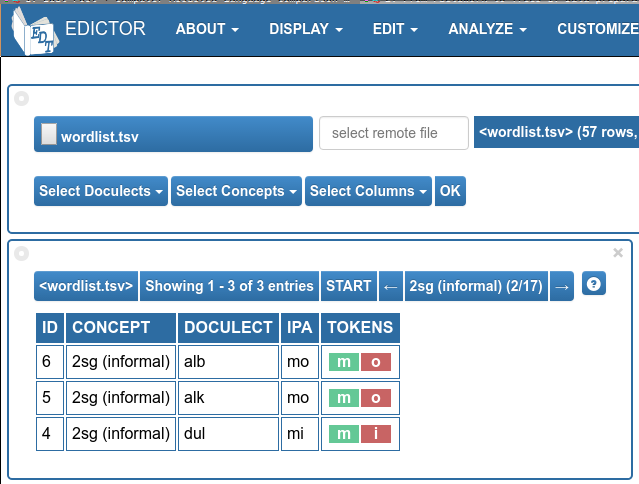
\includegraphics[width=10cm]{images/alorese.png}
\caption*{\small \textbf{Figure 1}: Forms 4--6 from wordlist.tsv in Edictor.}
\end{figure}

In order to make this script re-useable, it is obviously useful to
replace the hard-coded assumptions (file paths, separators, number of
gloss languages) with command line arguments and such like. If we want
to use LingPy for cognate coding, we also have to skip empty forms like
7--9 above with an \lstinline!if not form: continue! . But the core of
the conversion are just the last 10-or-so lines of this script, and then
I have my colleague's language in a format ready for further use, and
how I use it will be content of a later post.


\subsection*{References}

\nopagebreak\hangindent=0.7cm {\small List, Johann-Mattis \& Greenhill, Simon J. \& Forkel, Robert. 2018.
\emph{LingPy. A Python Library for Quantitative Tasks in Historical
Linguistics. Version 2.6.3}.  Zenodo. doi:
\href{https://doi.org/10.5281/zenodo.1203193.}{10.5281/zenodo.1203193.}
\url{https://zenodo.org/record/1203193\#.W-xUdhBRfc8} (14 November,
2018). }

\nopagebreak\hangindent=0.7cm {\small Forkel, Robert \& List, Johann-Mattis \& Greenhill, Simon J. \&
Rzymski, Christoph \& Bank, Sebastian \& Cysouw, Michael \&
Hammarström,~Harald \& Haspelmath, Martin \& Kaiping, Gereon A. \& Gray,
Russell D. 2018. Cross-Linguistic Data Formats, advancing data sharing
and re-use in comparative linguistics. \emph{Scientific Data} 5. 180205.
doi:
\href{https://doi.org/10.1038/sdata.2018.205}{10.1038/sdata.2018.205}. 
}

\vskip 2em
\framebox{\tabular{p{0.95\textwidth}}\textbf{Cite this article as}: Gereon A. Kaiping, \enquote{From
Fieldwork to Trees 1: Data preparation,} in \emph{Computer-Assisted
Language Comparison in Practice},  14/11/2018,
\url{https://calc.hypotheses.org/803}.\endtabular}
\newpage

\section*{Semantic promiscuity as a factor of productivity in word
formation}
\phantomsection\addcontentsline{toc}{section}{Semantic promiscuity as a factor of productivity in word
formation (Nathanael E. Schweikhard)}

Nathanael E. Schweikhard (19/11/2018)

\emph{Categories}: Terminology

\emph{Tags}: productivity, promiscuity, word formation

\begin{center}\rule{0.5\linewidth}{1pt}\end{center}

The blog post introduces ideas discussed in our project about taking a
closer look at word formation from a semantic (or semasiological) point
of view. Since this so far underinvestigated approach to word formation
processes lacks proper terminology, a new term to denote the central
research question of concept-based type-frequency is introduced and
contrasted with related established terminology.

\emph{Productivity} in the context of word formation is a term of many
definitions (Bauer 2003:1). A not necessarily exhaustive list is
provided by Gaeta and Ricca (2015), based on Rainer (1987):

\begin{enumerate}[a.] % (a), (b), (c), ...
\item the number of words formed with a certain W{[}ord {]}F{[}ormation
{]}R{[}ule{]};
\item the number of new words coined with a certain WFR in a given time
span;
\item the possibility of coining new words with a certain WFR;
\item the probability of coining new words with a certain WFR;
\item the number of possible (or generatable by rule) words formed with
a certain WFR;
\item the relation between occurring and possible words formed with a
certain WFR.
\end{enumerate}

Bauer (2003) mainly concerns himself with definitions c. to e., namely
to which degree a morphological pattern (i. e. what was above referred
to as a word formation rule) is available to be used in creating new
words, not how much it is actually used. According to him, this can be
determined by looking at the number of cases available for applying the
pattern, the number of (absolute or relative) constraints when applying
the pattern, and the usefulness of the word formations that it can
create.

Yet in either case, and in all the definitions given, the focus lies on
either the output side of word formation or on the restrictions of a
specific morphological pattern. These restrictions may lie in the input
(e. g. certain patterns only being applied to the input of specific
characteristics like for example a certain phonetic shape) but the
\emph{meaning} of the input itself has not been studied much so far,
although it is clear that word formation would not be possible without
it.

When investigating the semantics underlying word formation processes,
the general question from the perspective of the meaning of the input
could be stated as follows: \emph{Independent of any specific kind of
word formation pattern, are there morphemes that appear more commonly}
\emph{as bases of word formation than others, and if so, what do they
have in common?} In contrast to classical research on word formation,
which often investigates \emph{potential} word formations, this question
can probably best be studied by investigating \emph{existing} word
formation patterns, that is, by asking how often one morpheme occurs in
how many words (considering the whole lexicon of a given language, or a
certain section of it).

Shifting the focus from the forms to the concepts would also facilitate
cross-linguistic comparison, especially if one starts from basic
concepts, like the ones traditionally used in fieldwork and lexical
studies on historical language comparison (compare the Concepticon
resource,
\href{https://concepticon.clld.org/}{https://concepticon.clld.org}, for
an overview, List et al. 2016). Such research would, of course, not
assume that concepts are the same across languages, but rather employ
the idea of using \emph{comparative concepts} in the sense of Haspelmath
(2010:668).

Given that -- to my knowledge -- a systematic investigation of the
\enquote{semantic productivity} of concepts across languages has not
been carried out so far, we can only speculate why -- if at all -- some
words expressing specific concepts would recur more frequently as the
base of new words than others. Provided that we can identify
cross-linguistic trends, the Embodiment theory, according to which
language is shaped by our physical characteristics, might provide an
explanation. As one of the few studies devoted to the topic, Geisler
(2018) demonstrates for German that some of the morphemes denoting
concepts most deeply rooted in our early childhood experience (such as
\enquote{to stand} or \enquote{to fall}), seem to be used extremely
frequently in derivation for a large variety of meanings derived from
the conceptual base.

Unfortunately, there does not seem to be a proper term for what was
referred to as \enquote{semantic productivity} or ``concept-based
type-frequency`` above. Although the phenomenon by which a morpheme
reappears as part of word formations due to its semantics has been
sporadically mentioned and discussed before, no proper term has made it
into handbooks or glossaries of linguistics. The one who comes closest
to it is Blank (1997:21), who uses and slightly redefines the terms
\emph{attraction} and \emph{expansion} (coined by Sperber 1923) in order
to develop a theory of semantic change\footnote{My translation, original text: \enquote{Expansion und Attraktion
sind komplementäre Prozesse: Bei der Expansion handelt es sich um ein
semasiologisches Verfahren: Hier erhält ein Wort neue Bedeutungen. Die
Expansion kann somit auch bei der Erstbenennung von Neuerungen eine
wichtige Rolle spielen. Bei der Attraktion hingegen handelt es sich
primär um ein onomasiologisches Verfahren: Für ein und denselben
Sachverhalt werden neue Bezeichnungen geschaffen. Sekundär führt
natürlich auch die Attraktion zu Bedeutungswandel, nämlich bei den
Wörtern, die zur Bezeichnung des «attraktiven» Sachverhaltes
herangezogen wurden.}}:

\begin{quote}
Expansion and attraction are complementary processes: Expansion is a
semasiologic procedure: Here a word gains new meanings. Expansion
therefore can also play a role in the first-time denoting of an
innovation. Attraction on the other hand is primarily an onomasiologic
procedure: New denotions are created for one and the same concept.
Secundarily attraction of course also leads to semantic shift, namely in
those words that are used for denoting the «attractive» concept. (Blank
1997: 21)
\end{quote}

We can clearly see that Blank's term \emph{expansion} describes the
process underlying the phenomenon for which we do not yet have a name.
However, as Blank states himself, expansion is based on a semasiological
perspective: A specific word is gaining a new meaning additionally to
those it already had. Yet the phenomenon we discussed so far focuses on
an onomasiological approach that investigates how concepts contribute to
semantic expansions of the words denoting them. Furthermore, expansion
refers to a concrete process, situated in a specific language and time
frame, whereas our starting point was -- among others -- the question of
whether and to which degree universal tendencies could be encountered
when comparing the \enquote{expansivity} of concepts across the world's
languages.

Both expansion and what we are referring to here form counterparts to
Blank's term \emph{attraction}.  Attraction means that a concept
attracts new words or word formations denoting it. If, on the other
hand, a word's meaning expands, it can be used to coin new words, which
-- in turn -- would be expected to denote \enquote{attractive} concepts.

To form a wide range of new words, words first need to expand their
meaning, which itself is also based mainly on the meanings the words
already have. While meaning expansion can happen to any word independent
of its previous meanings, we here propose that some meanings might have
a stronger tendency to undergo this expansion.

After longer discussions in our project, during which we tested many
different terms as candidates to denote that some morphemes may be more
important for word formation due to their semantics, we decided to take
inspiration from microbiological terminology and use the term
\emph{promiscuity}.  Investigating the \emph{promiscuity of concepts},
be it cross-linguistically or within one language, would thus entail
that we investigate to what degree word formation is driven by the
semantics of the words or morphemes being recycled to form new words.

But why \enquote{promiscuity}? In the natural sciences, the term
\emph{promiscuity} has been used since at least the early 20th century
-- and more commonly since the 1970s -- as

\begin{quote}
{ {[}the{]} ability of a protein, organism, etc., to interact with a
variety of targets or in a non-specific manner; \emph{spec.} the
propensity of a plasmid, pathogenic organism, etc., to infect many
different hosts. (OED) }
\end{quote}

Given that biology and linguistics often share terminology and metaphors
(List et al. 2016a), we can also find examples in linguistics, where
promiscuity is used as a term, albeit it is less widespread and mainly
used in a quite restricted sense. Zwicky (1987:136), for example, speaks
of \enquote{promiscuous attachment} by which he means the
\enquote{attachment to i{[}nflected{]}-forms of virtually any syntactic
category} (he also uses the term \enquote{promiscuity} in Zwicky 1986
and talks about the same concept without having a term for it in Zwicky
and Pullum 1983). Similarly, Haspelmath (2018:315) uses
\enquote{promiscuous} for bound forms that attach to more than one word
class. In his definition, promiscuous morphemes form thus a category
between affixes and roots.

\begin{figure}[htb]
\centering
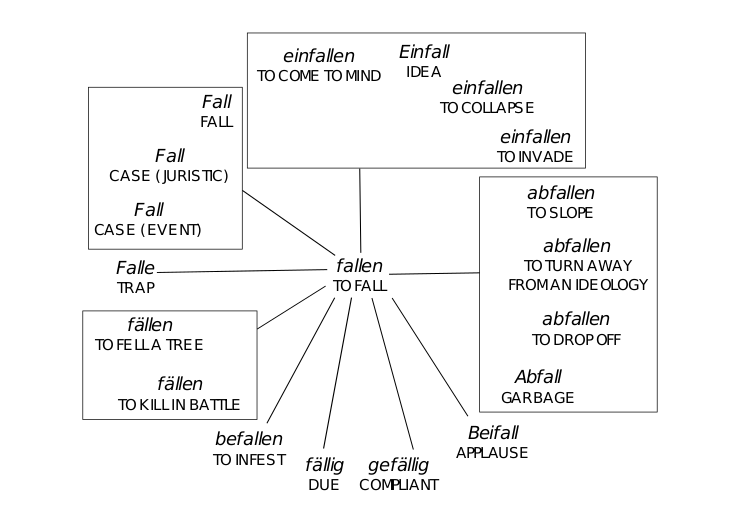
\includegraphics[width=0.8\textwidth]{images/fallen.png}
\captionsetup{justification=centering}
\caption*{\small \textbf{Figure 1:} The concept \enquote{to fall}, denoted by German
\emph{fallen}, showing its high promiscuity in a selection of the wide
range of meanings derived from it. This includes the expansion of
meanings of existing word formations, here marked by grouping together
derivations sharing the same stem. }
\end{figure}


In a slightly different approach, Zólyomi et al. (2017:21) use
\enquote{promiscuous} to refer to the mixing of cases, i. e. cases
extending their usage to functions previously inhabited by other cases.
However, they write this in the context of second language learners and
not of \enquote{normal} language change, and apparently do not intend to
use it as a technical term.

What all these uses of the term have in common is that they talk about
the \emph{openness} of something to connect to a variety of different
kinds of other things, a meaning that is clearly based on the term's
more colloquial usage.

The \emph{semantic promiscuity} proposed here (called such to
differentiate it from the more syntactic or grammatical concept by
Zwicky and Haspelmath) could first be said to differ from that original
meaning by being concerned with the type-frequency of a morpheme in
general, independent of its choice of word formation pattern or, e. g.,
of the grammatical variety of other morphemes it connects to.

However, while semantic promiscuity, unlike its grammatical counterpart,
is not referring to concepts being less restricted in the grammatical
aspects of the bases they can take, it nevertheless refers to something
similar, namely that morphemes denoting promiscuous concepts are less
restricted regarding the semantics of the morphemes they attach to in
word formation and the semantics of the new words formed thereby, either
by being already polysemous themselves, or by being more open to develop
polysemy, i. e. to undergo semantic expansion.

An example of how
promiscuity and expansion interact can be seen in Figure 1 above. Having
provided this preliminary description of what it is we are talking (or
want to talk) about, the next step will be to actually investigate it
cross-linguistically.

\subsection*{References}

\nopagebreak\hangindent=0.7cm {\small Bauer, Laurie. 2003. \emph{Morphological Productivity}.  Cambridge:
Cambridge University Press. }

\nopagebreak\hangindent=0.7cm {\small Blank, Andreas. 1997. \emph{Prinzipien des lexikalischen
Bedeutungswandels am Beispiel der romanischen Sprachen}.  Beihefte zur
Zeitschrift für romanische Philologie 285. Tübingen: Niemeyer. }

\nopagebreak\hangindent=0.7cm {\small Gaeta, Livio, and Davide Ricca. 2015. \enquote{Productivity.} In
\emph{Word-Formation: An International Handbook of the Languages of
Europe}, edited by Peter O. Müller, Ingeborg Ohnheiser, Susan Olsen,
and Franz Rainer, 22:842--858. Handbücher zur Sprach- und
Kommunikationswissenschaft 2. Berlin;New York: De Gruyter Mouton. }

\nopagebreak\hangindent=0.7cm {\small Geisler, Hans. 2018. \enquote{Sind Unsere Wörter von Sinnen?
Überlegungen zu den sensomotorischen Grundlagen der Begriffsbildung.} In
\emph{Worte über Wörter. Festschrift zu Ehren von Elke
Ronneberger-Sibold}, edited by Kerstin Kazzazi, Karin Luttermann,
Sabine Wahl, and Thomas A. Fritz, 131--142. Tübingen: Stauffenburg. }

\nopagebreak\hangindent=0.7cm {\small Haspelmath, Martin. 2010. \enquote{Comparative Concepts and
Descriptive Categories in Crosslinguistic Studies.} \emph{Language: A
Jou { rnal of the Linguistic Society of America }}, no. 86, 3:
663--687. }

\nopagebreak\hangindent=0.7cm {\small List, Johann-Mattis, Michael Cysouw, Simon J. Greenhill, and Robert
Forkel, eds. 2018. \emph{Concepticon}.  Jena: Max Planck Institute for
the Science of Human History. \url{http://concepticon.clld.org/}.  }

\nopagebreak\hangindent=0.7cm {\small List, Johann-Mattis, Michael Cysouw, and Robert Forkel. 2016.
\enquote{Concepticon. A Resource for the Linking of Concept Lists.} In
\emph{Proceedings of the Tenth International Conference on Language
Resources and Evaluation}, edited by Nicoletta Calzolari, Khalid
Choukri, Thierry Declerck, Marko Grobelnik, Bente Maegaard, Joseph
Mariani, Asuncion Moreno, Jan Odijk, and Stelios Piperidis, 2393--2400.
Portorož: European Language Resources Association. }

\nopagebreak\hangindent=0.7cm {\small List, Johann-Mattis, Jananan Sylvestre Pathmanathan, Philippe Lopez,
and Eric Bapteste. 2016. \enquote{Unity and Disunity in Evolutionary
Sciences: Process-Based Analogies Open Common Research Avenues for
Biology and Linguistics.} \emph{Biology Direct}.  }

\nopagebreak\hangindent=0.7cm {\small OED Online. July 2018. Oxford University Press.
\url{http://www.oed.com/view/Entry/152428?redirectedFrom=promiscuity}
(accessed November 16, 2018). }

\nopagebreak\hangindent=0.7cm {\small Rainer, Franz. 1987. \enquote{Grammatik und Wortbildung romanischer
Sprachen.} In \emph{Produktivitätsbegriffe in der Wortbildungslehre},
edited by Wolf Dietrich, Hans-Martin Gauger, and Horst Geckeler,
187--202. Tübingen: Narr. }

\nopagebreak\hangindent=0.7cm {\small Sperber, Hans. 1923. \emph{Einführung in die Bedeutungslehre}.  Bonn;
Leipzig: Schroeder. }

\nopagebreak\hangindent=0.7cm {\small Zólyomi, Gábor, Szilvia Jáka-Sövegjártó, and Melinda Hagymássy. 2017.
\emph{An Introduction to the Grammar of Sumerian}.  Budapest: Eötvös
University Press. }

\nopagebreak\hangindent=0.7cm {\small Zwicky, Arnold M. 1986. \enquote{Incorporating the Insight of
Autolexical Syntax.} \emph{OSU Working Papers in Linguistics} 32:
139--143. }

\nopagebreak\hangindent=0.7cm {\small Zwicky, Arnold M. 1987. \enquote{Suppressing the Zs.} \emph{Journal of
Linguistics} 23 (1): 133--148. \url{http://www.jstor.org/stable/4175870}
. }

\nopagebreak\hangindent=0.7cm {\small Zwicky, Arnold M., and Geoffrey K. Pullum. 1983. \enquote{Clitization
vs.~Inflection: English N'T.} \emph{Language} 59 (3): 502--513. }

\vskip 2em
\framebox{\tabular{p{0.95\textwidth}}\textbf{Cite this article as}: Nathanael E. Schweikhard,
\enquote{Semantic promiscuity as a factor of productivity in word
formation,} in \emph{Computer-Assisted Language Comparison in Practice}, 19/11/2018, \url{https://calc.hypotheses.org/1169}.\endtabular}

\newpage

\section*{From Fieldwork to Trees 2: Cognate coding}
\phantomsection\addcontentsline{toc}{section}{From Fieldwork to Trees 2: Cognate coding (Gereon A. Kaiping)}

Gereon A. Kaiping (27/11/2018)

\emph{Categories}: Code, Dataset

\emph{Tags}: Austronesian Languages, CLDF, code example, cognate
detection, cross-linguistic data formats, lexical data

\begin{center}\rule{0.5\linewidth}{1pt}\end{center}

In \href{https://calc.hypotheses.org/803}{a previous post} (Kaiping
2018), I described how to convert matrix-shape word lists given in Excel
into the long format LingPy and other software can work with. My
motivation for this was to provide my colleague Yunus Sulistyono with a
good way to compare the lexicon of his Alorese {[}
\href{https://glottolog.org/resource/languoid/id/alor1247}{alor1247} {]}
dialects, and to understand the relationship between them. In this post,
the data is automatically cognate coded and converted into CLDF.


If we have a file like the following, we can easily use LingPy's
functionality to get cognate classes.

\begin{table}[h]
\centering
\begin{tabular}{@{}lllll@{}}
\toprule
ID & CONCEPT        & DOCULECT & IPA & TOKENS \\ \midrule
1  & 1sg            & dul      & gɔ  & g ɔ    \\
2  & 1sg            & alk      & go  & g o    \\
3  & 1sg            & alb      & go  & g o    \\
4  & 2sg (informal) & dul      & mi  & m i    \\
5  & 2sg (informal) & alk      & mo  & m o    \\
6  & 2sg (informal) & alb      & mo  & m o    \\ \bottomrule
\end{tabular}
\captionsetup{justification=centering}
\caption*{\small \textbf{Table 1}: Sample of data from wordlist.tsv in tabular form.}
\label{tab:my-table}
\end{table}
 
This whole file (\lstinline!wordlist.tsv!) contains
data on dialects of one language (at least in simplified terms of the
self-identification of the speakers, who refer to all these varieties as
\enquote{bahasa Alor} -- how valid that categorization actually is might
be one outcome of his project) all transcribed by the same researcher,
so we should not expect a lot of problems from inconsistent
transcription or from cognates that cannot be recognized as such in the
data.

Some word boundaries are marked, so we can make use of them as morpheme
boundaries and use partial cognate coding. For that, we use LingPy's
\lstinline!Partial! class, with LexStat (List 2012) for getting
similarities and infomap~(Rosvall \& Bergstrom 2008) as cluster method.
Infomap, which seems to be a very good baseline cluster method for
cognate coding purposes~(List, Lopez \& Bapteste 2016) is not listed in
the current documentation of the \lstinline!partial_cluster! method, but
it is implemented. The \lstinline!fuzzy! keyword to the
\lstinline!Alignments! constructor below tells the alignment algorithm
to align the individual words (or, more generally, morphemes) of each
form instead of trying to align the forms globally. This tends to
improve the resulting alignments vastly.

\begin{lstlisting}
import lingpy
lex = lingpy.compare.partial.Partial(
  "wordlist.tsv")

lex.get_scorer(runs=10000)

lex.partial_cluster(
  method='lexstat',
  threshold=0.55,
  cluster_method="infomap",
  ref='partialids',
  verbose=True)

lex.get_scorer(runs=10000)
alm = lingpy.Alignments(lex, ref="partialids", fuzzy=True)
alm.align(method='progressive')
alm.output('tsv', filename='aligned',
  ignore='all', prettify=False)
\end{lstlisting}

If all goes well, this generates a file \lstinline!aligned.tsv! in the
current directory with the automatic partial cognate codes and
alignments.~ (One way this can go wrong is if we have not filtered out
empty forms in the generation of \lstinline!wordlist.tsv! .) ~This is
good for a one-shot run to get an overview over the data (eg. with
Edictor), but if we want to try out different thresholds and cluster
algorithms, it would be wise to cache the LexStat scorers (in particular
the \lstinline!bscorer! , which is expensive to calculate) somewhere.

The easiest way to cache the scorer -- although at the cost of a huge
overhead, because it also saves the whole word list (and in this case
also all its metadate) -- is by outputting the wordlist with scorer to a
tsv file. If we want to have the scorer cache in
\lstinline!lexstats.tsv!, we can replace the \lstinline!get_scorer! line
above by

\begin{lstlisting}
try:
  scorers_etc = lingpy.compare.lexstat.LexStat(
    "lexstats.tsv")
  lex.scorer = scorers_etc.scorer
  lex.cscorer = scorers_etc.cscorer
  lex.bscorer = scorers_etc.bscorer
except OSError:
  lex.get_scorer(runs=10000)
  lex.output('tsv', filename='lexstats', ignore=[])
\end{lstlisting}

This reads the scorers from that file if it can, and computes them
otherwise. This allows us to change threshold and cluster method without
having to re-calculate the scorers every time.

The file generated by this script, \lstinline!aligned.tsv! , is again a
TSV file (although it has minor issues in presence of line breaks and
quotation marks in cells, because the QLC interface used by LingPy
handles these things differently from the standard python CSV module --
luckily we do not have the \lstinline!Comments! column in which people
would be most likely to use these characters) and can be read in
Edictor.

\begin{figure}[htb]
\centering
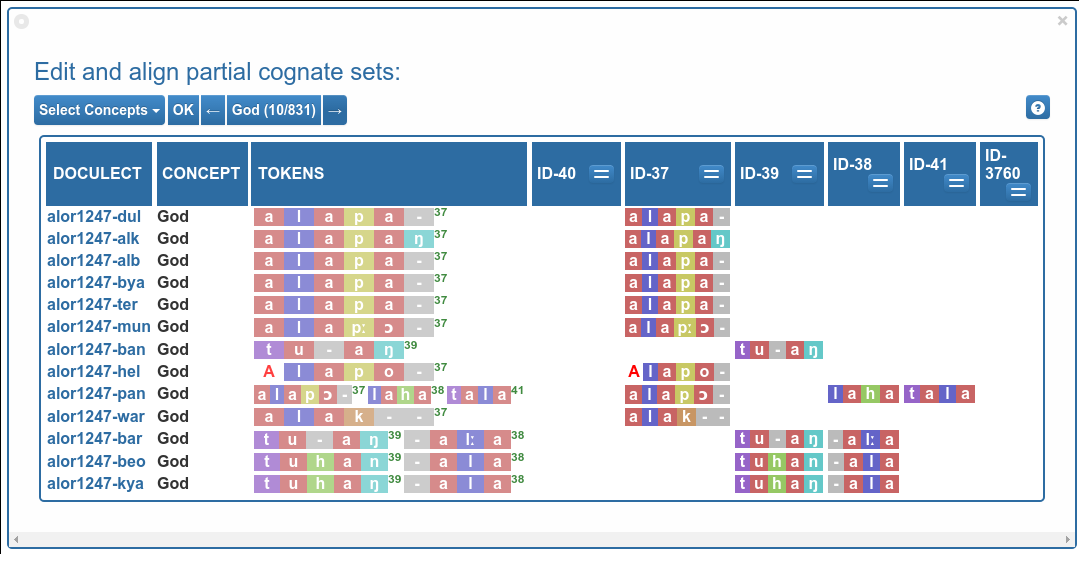
\includegraphics[width=10cm]{images/pcogs.png}
\captionsetup{justification=centering}
\caption*{\small \textbf{Figure 1}: Editing partial cognates in Edictor: The concept \enquote{God} in 13
varieties of Alorese}
\end{figure}

This screenshot also shows that the data is not entirely clean: The
\textless{}A\textgreater{} in the Helandohi form should not be
capitalized. For the gloss language Indonesian, which I have excluded
here, this is forgivable, because it was not intended as phonetic
transcription; for the actual forms, this shows we might have other
transcription errors, too.

While the file works nicely with LingPy and
Edictor, tools that follow the CLDF standard~(Forkel et al. 2018) -- of
which there are not many yet, but BEASTling (Maurits et al. 2017), which
I want to show in the following post, is one of them -- will not be able
to work with this file immediately. However, the standard is flexible
enough that we can transform this TSV file into valid CLDF very easily.
We just need to provide a JSON metadata file that describes the columns
in this data set. Implicitly, we know exactly which columns the TSV file
contains and what they mean in CLDF terms, so we can specify the
metadata as \href{https://calc.hypotheses.org/849}{demonstrated online}.

The source code, as well as a file containing the generic metadata for a
dataset like the above and, for reference, the specific metadata of
Yunus' dataset, are available
\href{https://github.com/Anaphory/matrix_to_beastling}{from Github}. 

\subsection*{References}

\nopagebreak\hangindent=0.7cm {\small Forkel, Robert \& List, Johann-Mattis \& Greenhill, Simon J. \&
Rzymski, Christoph \& Bank, Sebastian \& Cysouw, Michael \& Hammarström,
Harald \& Haspelmath, Martin \& Kaiping, Gereon A. \& Gray, Russell D.
2018. Cross-Linguistic Data Formats, advancing data sharing and re-use
in comparative linguistics. \emph{Scientific Data} 5. 180205. doi:
\href{https://doi.org/10.1038/sdata.2018.205}{10.1038/sdata.2018.205}. 
}

\nopagebreak\hangindent=0.7cm {\small Kaiping, Gereon Alexander. From Fieldwork to Trees 1: Data
preparation. 2018. Blogpost. \emph{Computer-Assisted Language Comparison
in Practice}.  \url{https://calc.hypotheses.org/803} (15 November,
2018). }

\nopagebreak\hangindent=0.7cm {\small List, Johann-Mattis. 2012. LexStat: Automatic detection of cognates in
multilingual wordlists. \emph{Proceedings of the EACL 2012 Joint
Workshop of LINGVIS \& UNCLH} (EACL 2012), 117--125. Stroudsburg, PA,
USA: Association for Computational Linguistics.
\url{http://dl.acm.org/citation.cfm?id=2388655.2388671} (12 August,
2015). }

\nopagebreak\hangindent=0.7cm {\small List, Johann-Mattis \& Lopez, Philippe \& Bapteste, Eric. 2016. Using
sequence similarity networks to identify partial cognates in
multilingual wordlists. \emph{Proceedings of the 54th Annual Meeting of
the Association for Computational Linguistics (Volume 2: Short Papers)},
vol.~2, 599--605. }

\nopagebreak\hangindent=0.7cm {\small Maurits, Luke \& Forkel, Robert \& Kaiping, Gereon A. \& Atkinson,
Quentin D. 2017. BEASTling: A software tool for linguistic phylogenetics
using BEAST 2. \emph{PLOS ONE} 12(8). e0180908. doi:
\href{https://doi.org/10.1371/journal.pone.0180908}{10.1371/journal.pone.0180908}.
}

\nopagebreak\hangindent=0.7cm {\small Rosvall, Martin \& Bergstrom, Carl T. 2008. Maps of random walks on
complex networks reveal community structure. \emph{Proceedings of the
National Academy of Sciences} 105(4). 1118--1123. doi:
\href{https://doi.org/10.1073/pnas.0706851105}{10.1073/pnas.0706851105}
. }

\vskip 2em
\framebox{\tabular{p{0.95\textwidth}}\textbf{Cite this article as}: Gereon A. Kaiping, \enquote{From
Fieldwork to Trees 2: Cognate coding,} in \emph{Computer-Assisted
Language Comparison in Practice}, 27/11/2018,
\url{https://calc.hypotheses.org/849}.\endtabular}

\newpage
\section*{Merging datasets with LingPy and the CLDF curation framework}
\phantomsection\addcontentsline{toc}{section}{Merging datasets with LingPy and the CLDF curation framework
(Johann-Mattis List)}

Johann-Mattis List (10/12/2018)

\emph{Categories}: Code, Dataset

\emph{Tags}: CLDF, Concepticon, EDICTOR, LingPy

\begin{center}\rule{0.5\linewidth}{1pt}\end{center}

Imagine you have two different datasets, both containing approximately
the same concepts, but slightly different numbers of columns and ---
more importantly --- potentially identical identifiers in the first
column. A bad idea for merging these datasets would be to paste them in
Excel or some other kind of spreadsheet software, and then trying to
manually adjust all problems that might occur during this process.

A better idea is to just use LingPy and our CLDF curation framework
(which was, for example, used when
establishing the CLICS² database, see
\href{http://bibliography.lingpy.org?key=List2018f}{List et al. 2018}),
which is basically not much work, requiring just a few lines of code to
be written, but giving you also the possibility to re-use these code
pieces on similar tasks.

I want to illustrate how this can be done by showing for two datasets (\href{http://bibliography.lingpy.org?key=Chacon2017}{Chacon 2017} and
\href{///home/mattis/projects/blogposts/calc-7-merging/Chacon2018}{Chacon
et al. forthcoming}), which are both curated within our CLDF framework,
how one can merge them with LingPy. Before we can start, we will install
these two datasets via \lstinline!pip! .

\begin{lstlisting}
$ pip install -e git+https://github.com/lexibank/chaconarawakan.git@v1.0.1#egg=lexibank_chaconarawakan
$ pip install -e git+https://github.com/lexibank/chaconbaniwa.git@v1.0.0#egg=lexibank_chaconbaniwa
\end{lstlisting}

In our Python script, we then load the two packages along with LingPy
and the \lstinline!pyconcepticon! package.

\begin{lstlisting}
from lingpy import *
from lexibank_chaconarawakan import Dataset as ds1
from lexibank_chaconbaniwa import Dataset as ds2
from pyconcepticon.api import Concepticon
\end{lstlisting}

\hyperdef{}{markdown}{}
Along with these packages, the LingPy packages will also have been
installed, if it was not already present on your computer. Both datasets
contain a \lstinline!raw! folder in which we find the original data as
it was curated within the EDICTOR/LingPy approach, that is: the data was
originally analyzed with LingPy (\href{http://bibliography.lingpy.org?key=List2018i}{List et al. 2018})
and then manually corrected with EDICTOR (\href{http://bibliography.lingpy.org?key=List2017d}{List 2017}). So
instead of loading the data with LingPy's CLDF reader, we load it in its
raw form, for convenience.

\begin{lstlisting}
wl1 = Wordlist(
    ds1().raw.joinpath(
        "arawakan_swadesh_100_edictor.tsv").as_posix()) 
wl2 = Wordlist(
    ds2().raw.joinpath(
        "Bruzzi_Granadillo.txt").as_posix())
\end{lstlisting}

\hyperdef{}{markdown}{}
The part of the data we want is the common Swadesh-list of 100 concepts
(\href{http://bibliography.lingpy.org?key=Swadesh1955}{Swadesh 1955}).
We load this list with help of the \lstinline!pyconcepticon! API,
published as part with the Concepticon project (\href{http://bibliography.lingpy.org?key=List2016a}{List et al. 2016}).

\begin{lstlisting}
swad = [
    c.concepticon_id for c in Concepticon(
        ).conceptlists['Swadesh-1955-100'].concepts.values()]

concepts = {
    wl2[idx, 'concept'] for idx in wl2 if wl2[
        idx, 'concepticon_id'] in swad}
\end{lstlisting}

\hyperdef{}{markdown}{}
We now declare a dictionary in Python to store the data that we want to
then write to a LingPy-wordlist file (that can also be read in edictor).
We use the columns present in the first wordlist as our standard, and
add two more, one for the original index (called \lstinline!old_idx!)
and one for a combined cognate-identifier (called \lstinline!cog!).

\begin{lstlisting}
D = {0: wl1.columns+['old_idx', 'cog']}
\end{lstlisting}

We now iterate over both wordlists and add the relevant entries to the
dictionary, making sure to separate the cognate-identifiers from each
other by assigning them to different sets (with help of the name of the
datasets that we add as part of the cognate-set identifier).

\begin{lstlisting}
nidx = 1
for idx in wl1:
    D[nidx] = [wl1[idx, h] for h in wl1.columns
        ] + ['chaconarawakan-'+str(idx)]
    D[nidx] += ['chaconarawakan-'+str(
        wl1[idx, 'cogid'])]
    nidx += 1
for idx in wl2:
    D[nidx] = [wl2[idx, h] for h in wl1.columns
        ] + ['chaconbaniwa-'+str(idx)]
    D[nidx] += ['chaconbaniwa-'+str(
        wl2[idx, 'cogid'])]
    nidx += 1
\end{lstlisting}

All that's left to do now is load the data in to a \lstinline!Wordlist!
object provided by LingPy and write it to file (after a few operations).

\begin{lstlisting}
wl = Wordlist(D)
\end{lstlisting}

First, we \lstinline!renumber! the cognates in the column
\lstinline!cog! in order to make sure they are numeric.

\begin{lstlisting}
wl.renumber('cogx', 'cogid', override=True)
\end{lstlisting}

Then, we segment the so far non-segmented entries in the data:
\lstinline!for idx, ipa, segments in wl.iter_rows('ipa', 'segments'):            if not segments:            wl[idx, 'segments'] = ipa2tokens(ipa)!

Now, we write all entries to file that conform to a concept that is also
present in Swadesh's list of 100 items.

\begin{lstlisting}
wl.output(
    'tsv', 
    filename='chacon-arawakan-baniwa', 
    subset=True, 
    cols=[
        c for c in wl.columns if c not in [
            'value_in_source']],
    rows=dict(
        concept = 'in '+str(concepts))
    )
\end{lstlisting}

This is essentially all. The data in file
\lstinline!chacon-arawakan-baniwa.tsv! can now be analyzed with LingPy
or also manually annotated with EDICTOR.

\subsection*{References}

\nopagebreak\hangindent=0.7cm {\small Chacon, T. (2017): Arawakan and Tukanoan contacts in Northwest
Amazonia prehistory. \emph{PAPIA} 27.2. 237-265.. }

\nopagebreak\hangindent=0.7cm {\small List, J.-M., M. Cysouw, and R. Forkel (2016): Concepticon. A resource
for the linking of concept lists. In: Proceedings of the Tenth
International Conference on Language Resources and Evaluation.
2393-2400. }

\nopagebreak\hangindent=0.7cm {\small List, J.-M. (2017): A web-based interactive tool for creating,
inspecting, editing, and publishing etymological datasets. In:
Proceedings of the 15th Conference of the European Chapter of the
Association for Computational Linguistics. System Demonstrations. 9-12.
}

\nopagebreak\hangindent=0.7cm {\small List, J.-M., S. J. Greenhill, C. Anderson, T. Mayer, T. Tresoldi, and R.
Forkel (eds.) (2018): CLICS: Database of Cross-Linguistic
Colexifications. Max Planck Institute for the Science of Human History:
Jena. \href{//clics.clld.org/”}{http://clics.clld.org/}.  }

\nopagebreak\hangindent=0.7cm {\small List, J.-M., S. J. Greenhill, T. Tresoldi, and R. Forkel (2018): LingPy.
A Python library for quantitative tasks in historical linguistics. Max
Planck Institute for the Science of Human History: Jena.
\href{//lingpy.org”}{http://lingpy.org}.  }

\nopagebreak\hangindent=0.7cm {\small Swadesh, M. (1955): Towards greater accuracy in lexicostatistic
dating. \emph{International Journal of American Linguistics} 21.2.
121-137. }

\vskip 2em
\framebox{\tabular{p{0.95\textwidth}}\textbf{Cite this article as}: Johann-Mattis List, \enquote{Merging
datasets with LingPy and the CLDF curation framework,} in
\emph{Computer-Assisted Language Comparison in Practice},  10/12/2018,
\url{https://calc.hypotheses.org/1668}.\endtabular}

\end{document}
